\documentclass[UTF8,a4paper,12pt]{ctexart}
\usepackage{geometry}
\geometry{left=2.45cm,right=2.45cm,top=2.45cm,bottom=2.45cm}
\usepackage{setspace}
\setstretch{1.36}
\usepackage{fancyhdr}
\pagestyle{fancy}
\fancyhf{}
\fancyhead[C]{\small 颜色与物质浓度辨识模型研究}
\fancyfoot[C]{\thepage}
\setlength{\headheight}{14pt}
\usepackage{amsmath,amssymb,bm,booktabs,array,graphicx,float,caption,hyperref,tocloft}
\setlength{\cftbeforesecskip}{2pt}
\captionsetup[table]{position=top}
\captionsetup[figure]{position=bottom}
\graphicspath{{../quest1/figures/}{../quest2/figures/}{../quest3/figures/}}
\title{\heiti\zihao{2} 基于白板校正色差与正则化回归的颜色--浓度辨识模型}
\author{}
\date{}
\begin{document}
\maketitle
\thispagestyle{empty}
\begin{center}\heiti 摘\quad 要\end{center}
比色法将待测物质与试纸反应后的颜色同标准比色卡比较来判定浓度档位，但人工读色受主观敏感性、照明和观测误差影响。本文以附件中 RGB/HSV 颜色读数为数据基础，建立颜色读数到物质浓度的定量辨识模型，并从数据质量、模型误差、数据量和颜色维度三个方面完成分析。所有关键数字均由 Python 程序复现并冻结在 \texttt{frozen\_numbers.json} 中。\par
针对问题一，本文将“水”样本作为零浓度白板基准，构造相对白板五维色差 $D_0$，再从单调性、相邻浓度可分性、重复测量稳定性和留一预测误差四个角度建立数据优劣评价准则。结果表明，五组数据并非都能稳定确定颜色读数与浓度之间的一一关系，其中溴酸钾综合质量分最高，为 91.64；工业碱和组胺分别为 91.09、89.41；奶中尿素综合质量分最低，仅为 52.91，颜色变化幅度小、浓度档间重叠明显。\par
针对问题二，本文对 Data2 中二氧化硫数据建立多模型比较体系，以 $D_0$ 一元线性回归为 baseline，并比较 RGB 岭回归、HSV 岭回归、五维岭回归、五维二次岭回归和 PLS 回归。采用留一交叉验证评价小样本泛化误差。最优模型为五维二次岭回归，留一 RMSE 为 10.25 ppm，MAE 为 6.17 ppm，MAPE 为 9.75\%，$R^2$ 为 0.960；相比 baseline 的 RMSE=13.71 ppm，误差降低约 25.3\%。\par
针对问题三，本文通过样本子抽样、颜色维度消融和读数噪声扰动讨论数据规模与维度的影响。完整样本下，RGBSH 五维模型 RMSE 为 10.60 ppm，优于 D0、RGB 和 HSV 单独建模；置换重要性显示 H 维度贡献最高。当颜色读数附加噪声标准差由 0 增至 5 时，RMSE 从 10.60 ppm 增至 23.73 ppm，说明实际使用时应增加重复样本并统一光照与白平衡。\par
\noindent\textbf{关键词：} 比色法；颜色空间；白板校正；岭回归；留一交叉验证
\newpage
\tableofcontents
\newpage
\section{问题重述}
\subsection{问题背景}
比色法是一类常见的现场快速检测方法。待测溶液滴加到白色试纸表面后，试纸中的显色剂与待测物发生反应，最终呈现与物质浓度相关的颜色。传统做法是把显色后的试纸与标准比色卡进行肉眼比对，从而得到待测物的浓度档位。该方法成本低、速度快，适合食品安全、环境监测和快速筛查等场景；但其缺点也很明显：不同人员对色差的敏感度不同，拍照角度、光照条件和仪器白平衡会导致颜色读数偏移，人工判读也难以给出连续浓度。

随着数码相机和移动终端颜色分辨率提高，若能将照片中的颜色读数转化为浓度，则可以把定性比色卡升级为定量读数模型。附件 Data1 给出五种物质在若干浓度下的颜色读数，Data2 给出二氧化硫在若干浓度下的颜色读数。颜色读数包含 RGB 与 HSV 中的多个维度，其中不同维度对浓度的响应强弱和稳定性不同，不能简单假设任意一种颜色通道都能准确反映浓度。因此需要先判断数据本身是否足以支持建模，再选择合适的回归模型并分析误差。
\subsection{问题要求}
本文将题目要求拆解为三个子问题：一是对 Data1 中五种物质判断颜色读数与浓度之间能否确定数量关系，并给出评价优劣的准则；二是对 Data2 中二氧化硫数据建立颜色读数到物质浓度的数学模型，并给出误差分析；三是探讨数据量和颜色维度对模型的影响。本文分别输出数据质量评分、最优预测模型和实验设计建议。
\section{问题分析}
\subsection{总体思路}
本题属于小样本多变量回归与数据质量评价问题。颜色读数随浓度变化并不一定线性，且不同物质的显色机理、反应范围和读数噪声不同，所以不能直接把五组数据合并成一个通用模型。本文采用“先评价数据，再针对待建模物质建立回归模型，最后做数据量与维度影响分析”的路线。

整体流程为：首先读取并整理 Excel 附件，把“水”统一视为零浓度基准；其次以零浓度样本的颜色均值作为白板基准，计算样本与白板的相对色差；再次从单调性、可分性、重复性和可预测性评价 Data1；然后在 Data2 上建立一元色差 baseline 和多维正则化回归模型，使用留一交叉验证比较误差；最后通过子抽样和维度消融分析模型对样本量、颜色维度和读数噪声的依赖。
\subsection{问题一分析}
问题一的关键不是直接求某个浓度，而是判断一组颜色数据是否支持稳定定量关系。若颜色指标随浓度单调变化、不同浓度档之间的均值距离大于组内波动、重复测量稳定，则可以认为该物质具备较好建模基础；反之，即使训练集上可以拟合出公式，也可能是偶然拟合，难以推广。本文构造单调性、相邻可分性、重复稳定性和可预测性四类准则。
\subsection{问题二分析}
Data2 的建模对象是二氧化硫浓度。样本量只有 25 个，浓度水平为 0、20、30、50、80、100、150 ppm，属于典型小样本回归问题。若直接使用复杂机器学习模型，很容易过拟合；若只用单一颜色维度，又可能忽略多通道信息。因此本文设置相对白板色差 $D_0$ 的一元线性回归作为 baseline，再比较 RGB、HSV、RGBSH 五维和二次特征的正则化模型。
\subsection{问题三分析}
数据量和颜色维度是决定比色模型精度的两类核心因素。数据量不足时，模型参数估计不稳定，尤其高维或二次项模型会显著增加自由度；颜色维度不足时，模型可能丢失显色变化信息，颜色维度过多时又可能引入冗余噪声。因此需要同时考察样本数量和维度组合。
\section{数据来源、预处理与模型假设}
\subsection{数据来源与字段说明}
原始数据来自题目附件 Data1.xls 和 Data2.xls。Data1 包含五种物质：组胺、溴酸钾、工业碱、硫酸铝钾、奶中尿素；Data2 包含二氧化硫不同浓度下的颜色读数。清洗后 Data1 有 48 个有效样本、5 种物质；Data2 有 25 个有效样本，浓度水平为 0、20、30、50、80、100、150 ppm。Excel 中用于分组的空行和合并单元格样式不作为有效样本；水样统一编码为 0 ppm。清洗后所有建模字段无缺失值。
\subsection{预处理方法}
设样本 $i$ 的颜色向量为 $\bm x_i$。对每种物质，取零浓度水样的颜色均值为白板基准 $\bar{\bm x}_0$。定义相对白板色差
\begin{equation}
D_i=\|\bm x_i-\bar{\bm x}_0\|_2=\sqrt{\sum_{j=1}^p(x_{ij}-\bar x_{0j})^2}.
\end{equation}
对于回归模型，因浓度非负且变化范围较大，本文对目标变量采用 $z_i=\log(1+c_i)$ 建模，预测后再用 $\hat c_i=\exp(\hat z_i)-1$ 还原，最后将负预测截断为 0。
\subsection{模型假设}
（1）附件颜色读数由同类拍照或读色条件获得，除随机噪声外不存在系统性标注错误；（2）同一物质内颜色随浓度变化具有稳定响应趋势，但不同物质显色机制不同；（3）水样可代表零浓度白板基准；（4）短时间内拍照读数误差可视为独立扰动。这些假设分别服务于回归建模、分物质评价、白板校正和噪声敏感性分析。
\section{符号说明}
\begin{table}[H]\centering\caption{主要符号说明}\begin{tabular}{lll}\toprule
符号 & 含义 & 单位/说明\\\midrule
$c_i$ & 第 $i$ 个样本真实浓度 & ppm\\
$\hat c_i$ & 模型预测浓度 & ppm\\
$\bm x_i$ & 第 $i$ 个样本颜色读数向量 & RGB/HSV 读数\\
$\bar{\bm x}_0$ & 零浓度水样平均颜色向量 & 白板基准\\
$D_i$ & 相对白板色差 & 颜色读数距离\\
$\rho$ & Spearman 秩相关系数 & 无量纲\\
$\lambda$ & 岭回归正则化系数 & 无量纲\\
$e_i$ & 残差 $c_i-\hat c_i$ & ppm\\
\bottomrule\end{tabular}\end{table}
\section{模型建立与求解}
\subsection{问题一：五组数据质量评价模型}
题目要求讨论 Data1 中五组数据能否确定颜色读数和浓度之间的关系，并给出评价优劣的准则。本文模型输出四个评价维度及综合质量分。单调性指标为 $M=\max_j |\rho(c,x_j)|$；相邻可分性指标为
\begin{equation}
S_k=\frac{\|\bar{\bm x}_{k+1}-\bar{\bm x}_k\|_2}{s_{k+1}+s_k+\varepsilon},\quad Q=35M+25\tanh(\bar S/2)+25(1-\min(\mathrm{MAPE},100)/100)+15(1-r/15)_+ .
\end{equation}
\begin{table}[H]\centering\small\caption{Data1 五组数据质量评价结果}\begin{tabular}{lrrrr}\toprule
物质 & Spearman & 可分性 & MAPE(\%) & 综合分\\\midrule
溴酸钾 & 1.000 & 5.895 & 11.72 & 91.64\\
工业碱 & 1.000 & 5.192 & 2.63 & 91.09\\
组胺 & 1.000 & 5.073 & 4.95 & 89.41\\
硫酸铝钾 & 1.000 & 2.000 & 0.00 & 73.00\\
奶中尿素 & 0.919 & 1.392 & 75.47 & 52.91\\
\bottomrule\end{tabular}\end{table}
由表可知，溴酸钾综合质量分最高，说明其颜色读数随浓度变化具有较强单调性，且相邻浓度之间可分性较好。工业碱的得分与溴酸钾接近，颜色变化幅度大，适合建立定量模型。组胺也表现出较好的单调性和预测能力。奶中尿素得分最低，主要原因是颜色变化弱、不同浓度档间重叠明显。
\begin{figure}[H]\centering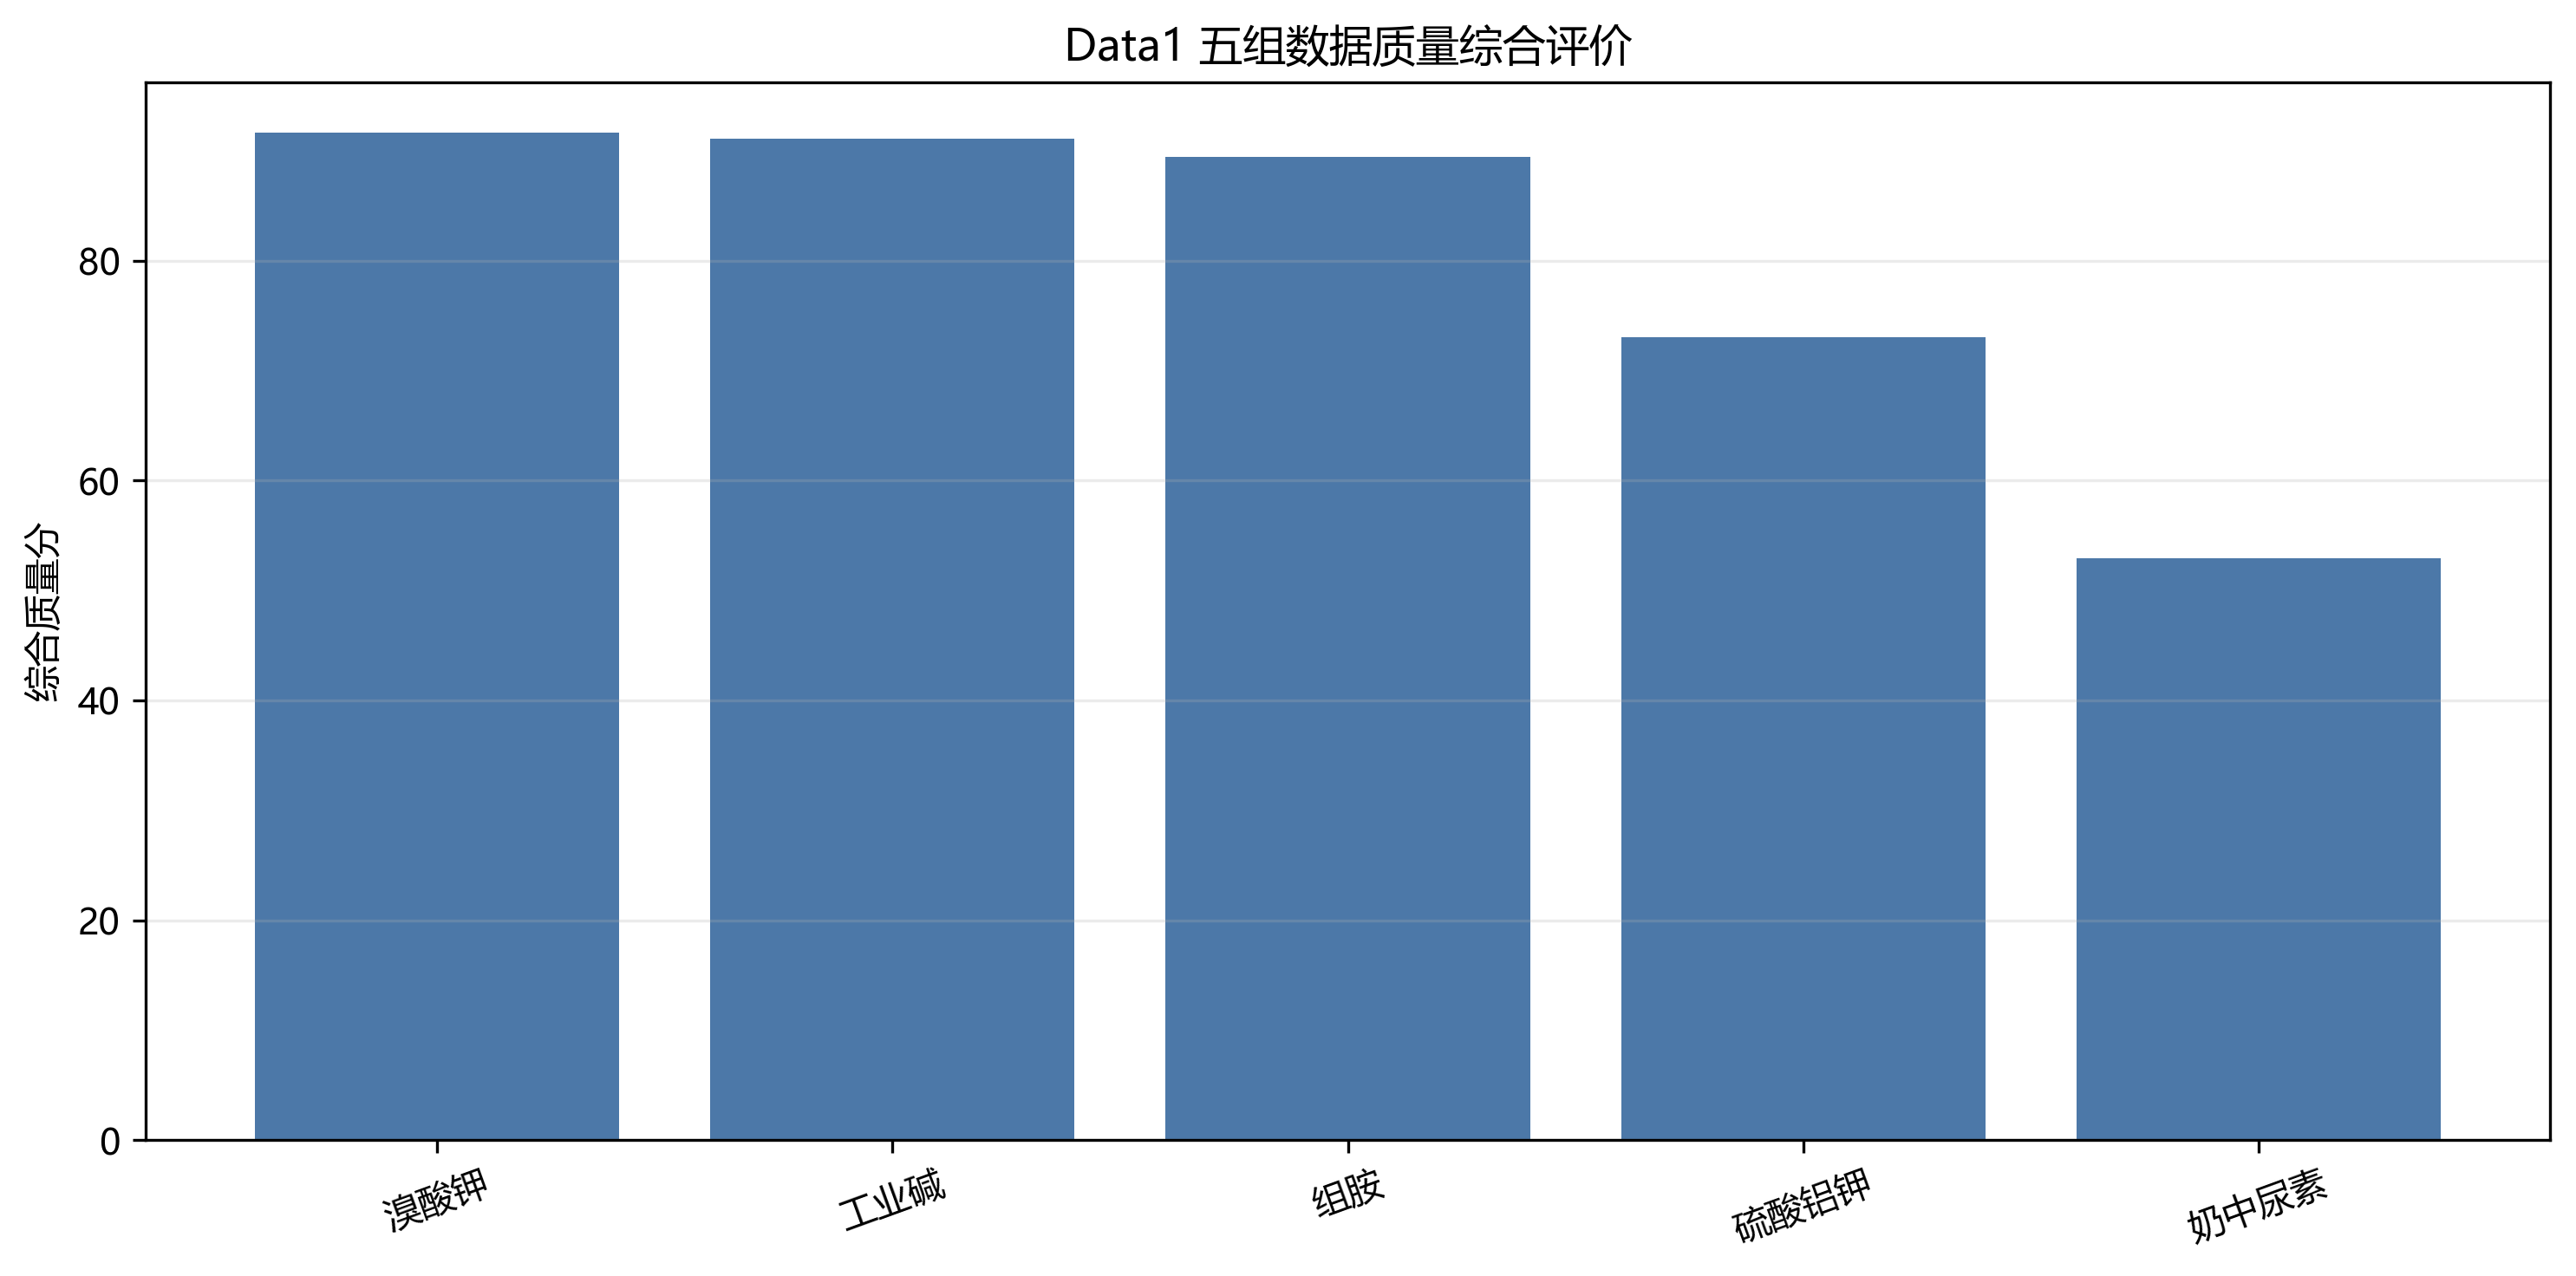
\includegraphics[width=.88\textwidth]{问题1_五组数据质量评分.png}\caption{五组数据综合质量评分}\end{figure}
\begin{figure}[H]\centering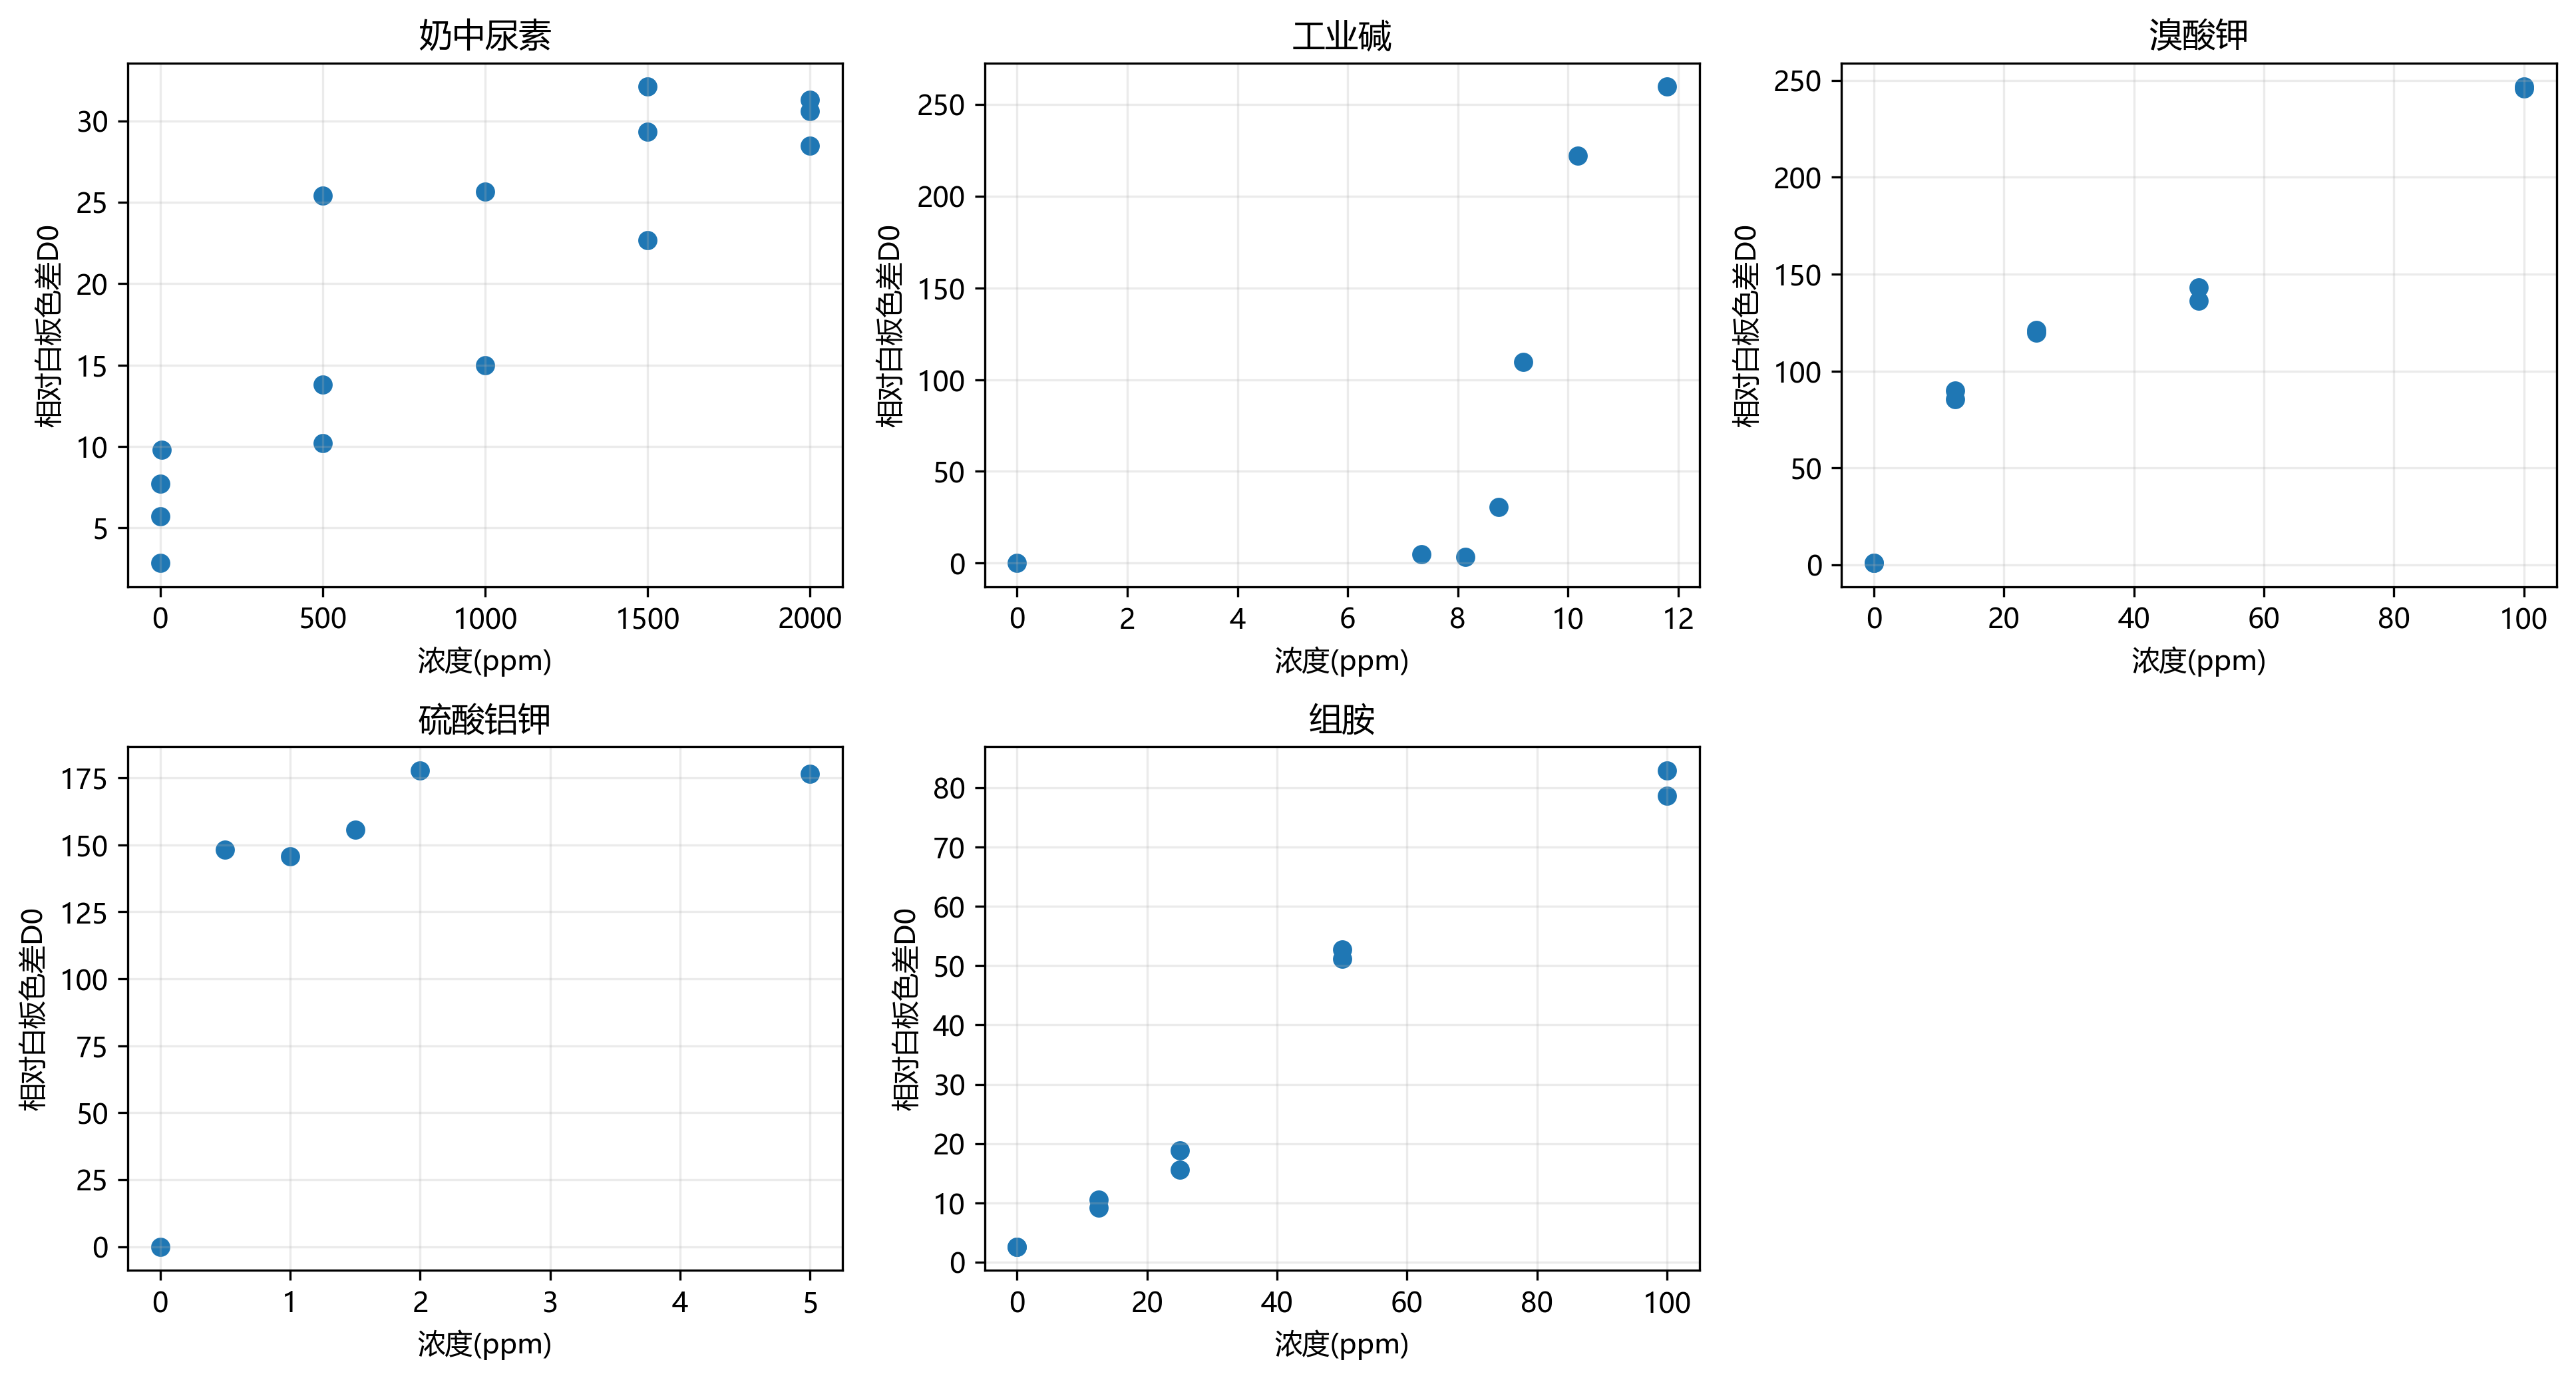
\includegraphics[width=.96\textwidth]{问题1_色差浓度关系散点图.png}\caption{相对白板色差与浓度关系散点图}\end{figure}
两张图共同说明，同样是比色数据，不同物质的显色响应质量差异很大，不能只凭有颜色读数就认为一定能建立可靠模型。
\subsection{问题二：二氧化硫颜色--浓度回归模型}
Baseline 只使用相对白板色差 $D$ 建立一元线性回归：$\log(1+c_i)=\beta_0+\beta_1D_i+\epsilon_i$。主模型采用五维二次岭回归：
\begin{equation}
\log(1+c_i)=\beta_0+\sum_j\beta_jx_{ij}+\sum_{j\le k}\gamma_{jk}x_{ij}x_{ik}+\epsilon_i,\quad
\min_{\bm\theta}\sum_i(z_i-\hat z_i)^2+\lambda\|\bm\theta\|_2^2.
\end{equation}
候选模型均采用留一交叉验证，误差指标为 RMSE、MAE、MAPE 和 $R^2$。
\begin{table}[H]\centering\small\caption{Data2 候选模型留一交叉验证误差}\begin{tabular}{lrrrr}\toprule
模型 & RMSE & MAE & MAPE(\%) & $R^2$\\\midrule
FiveDim\_Poly2\_Ridge & 10.251 & 6.166 & 9.751 & 0.960\\
HSV\_Ridge & 12.629 & 7.989 & 15.879 & 0.939\\
Baseline\_D0\_Linear & 13.715 & 9.063 & 16.930 & 0.928\\
RGB\_Ridge & 15.298 & 10.429 & 21.413 & 0.910\\
RGBSH\_Ridge & 18.745 & 11.666 & 22.302 & 0.865\\
PLS\_2comp & 24.468 & 17.287 & 33.016 & 0.770\\
\bottomrule\end{tabular}\end{table}
表中显示，五维二次岭回归的 RMSE、MAE 和 MAPE 均最低。其 RMSE=10.25 ppm，相比 baseline 的 13.71 ppm 降低约 25.3\%。
\begin{figure}[H]\centering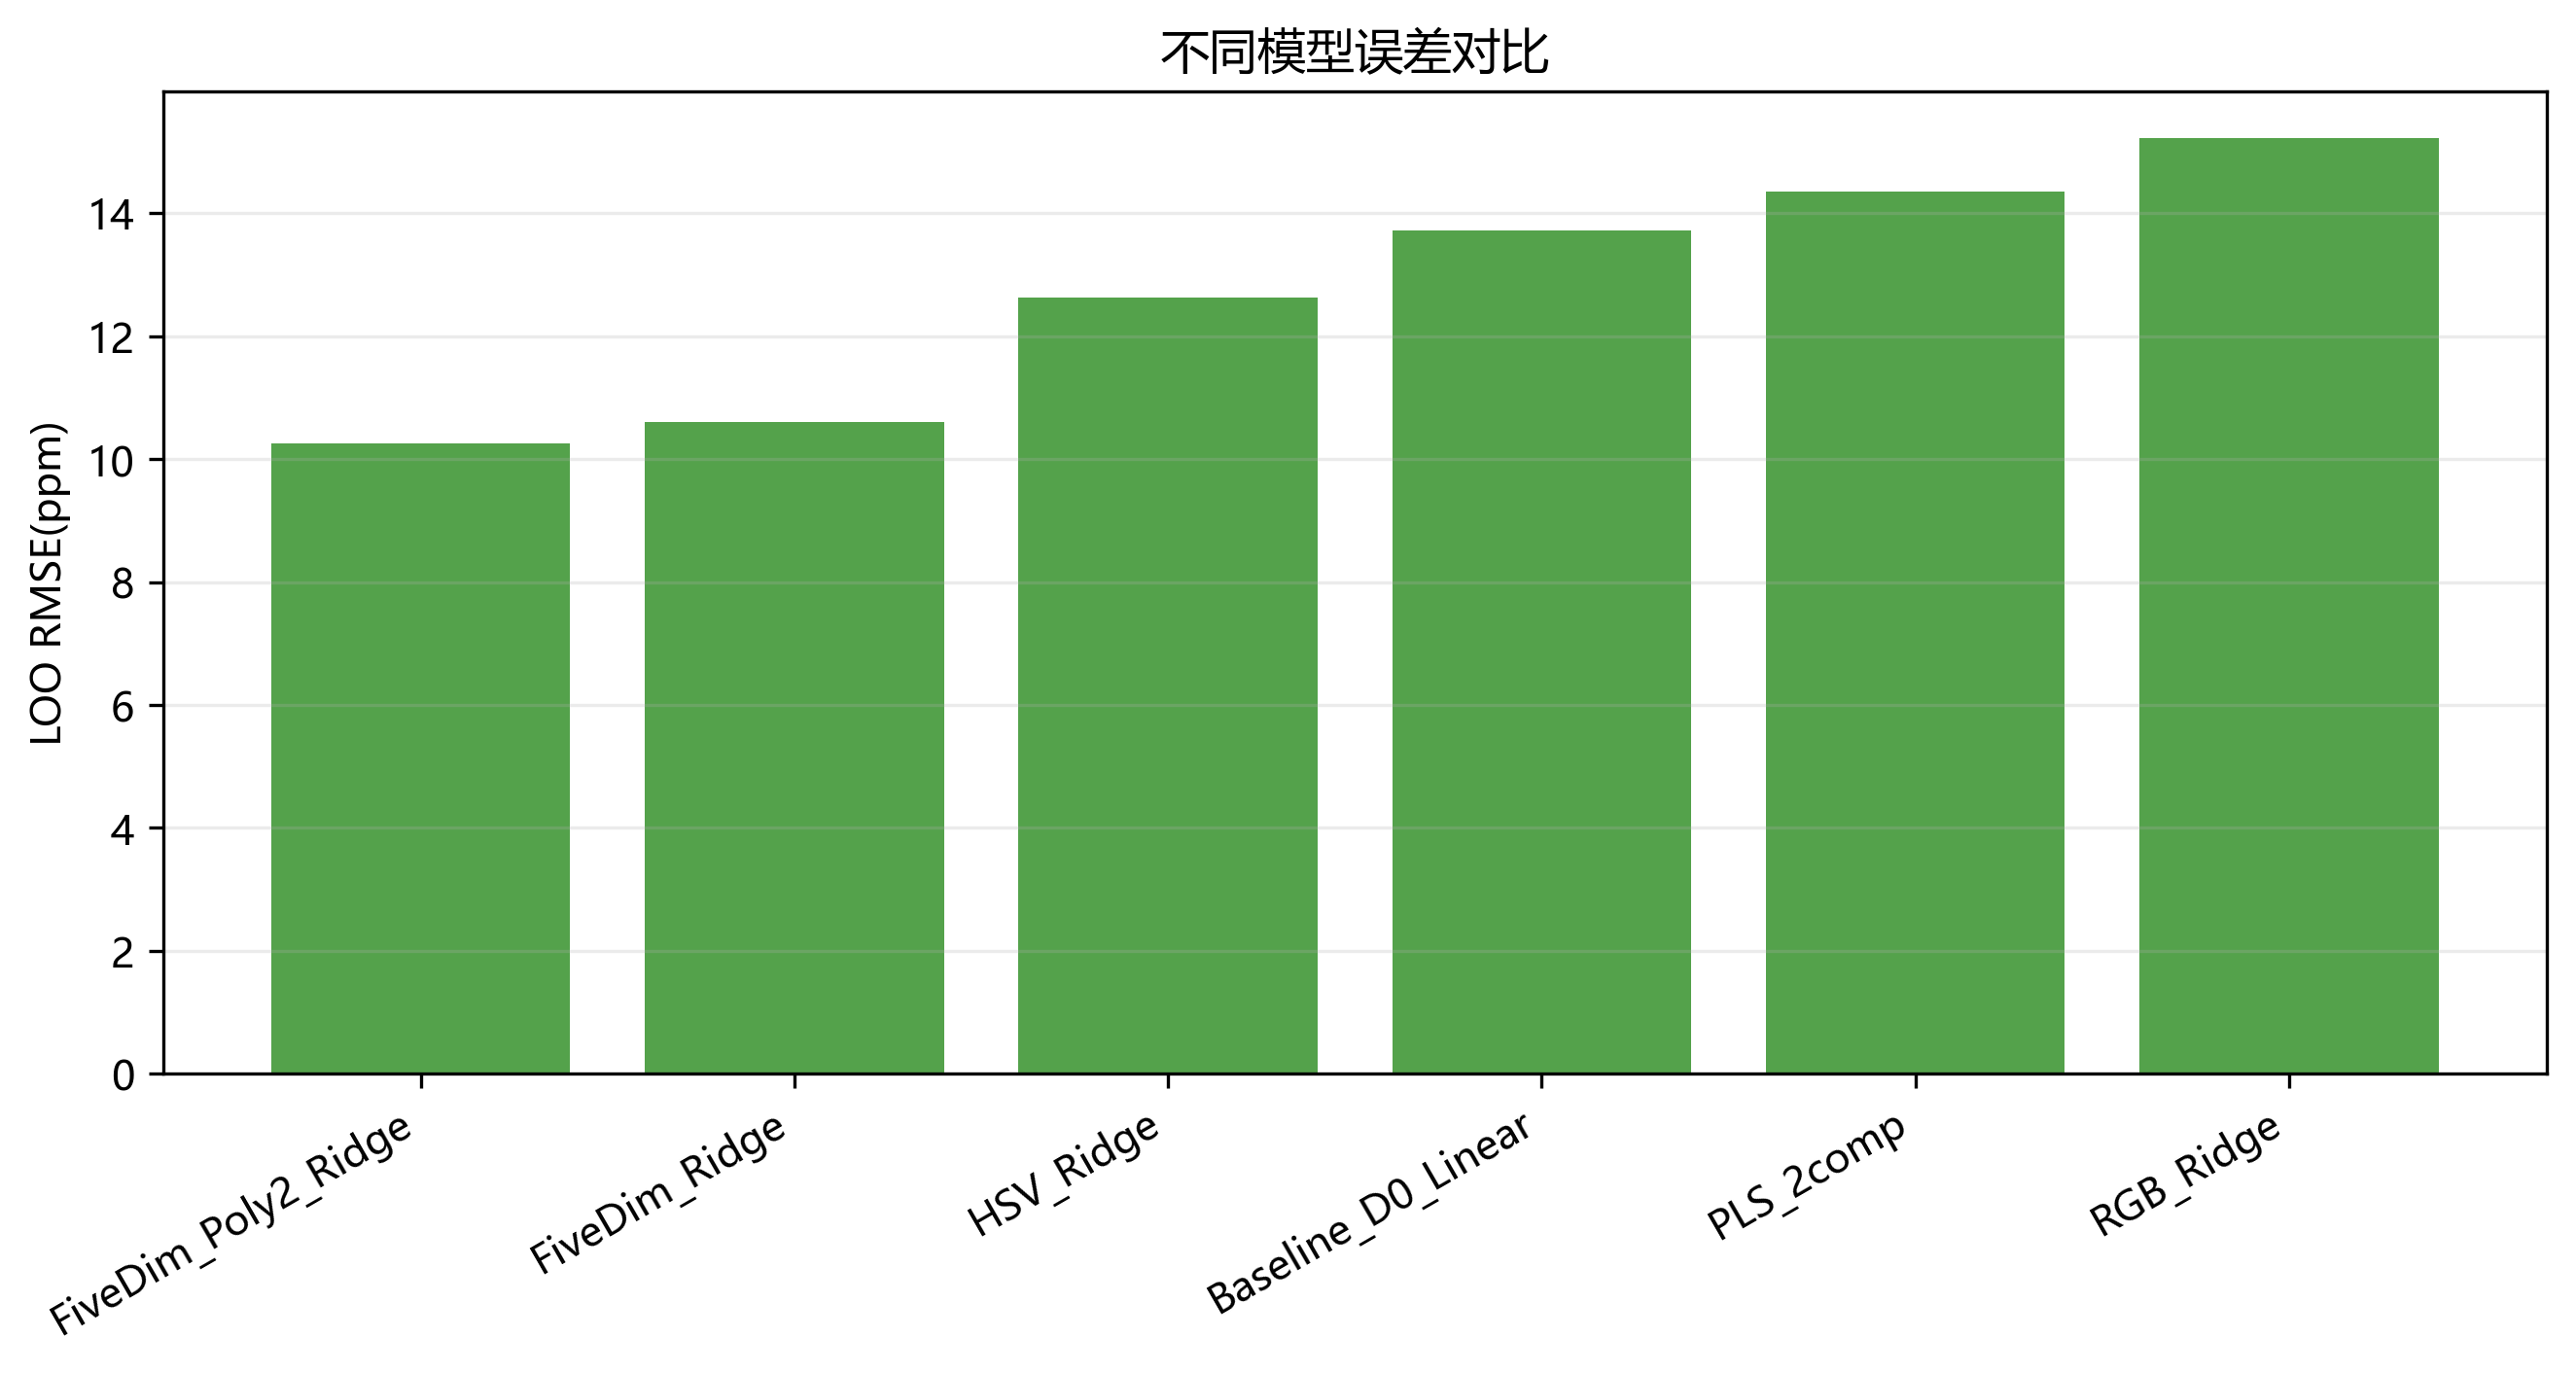
\includegraphics[width=.78\textwidth]{问题2_模型误差对比.png}\caption{候选模型 RMSE 对比}\end{figure}
\begin{figure}[H]\centering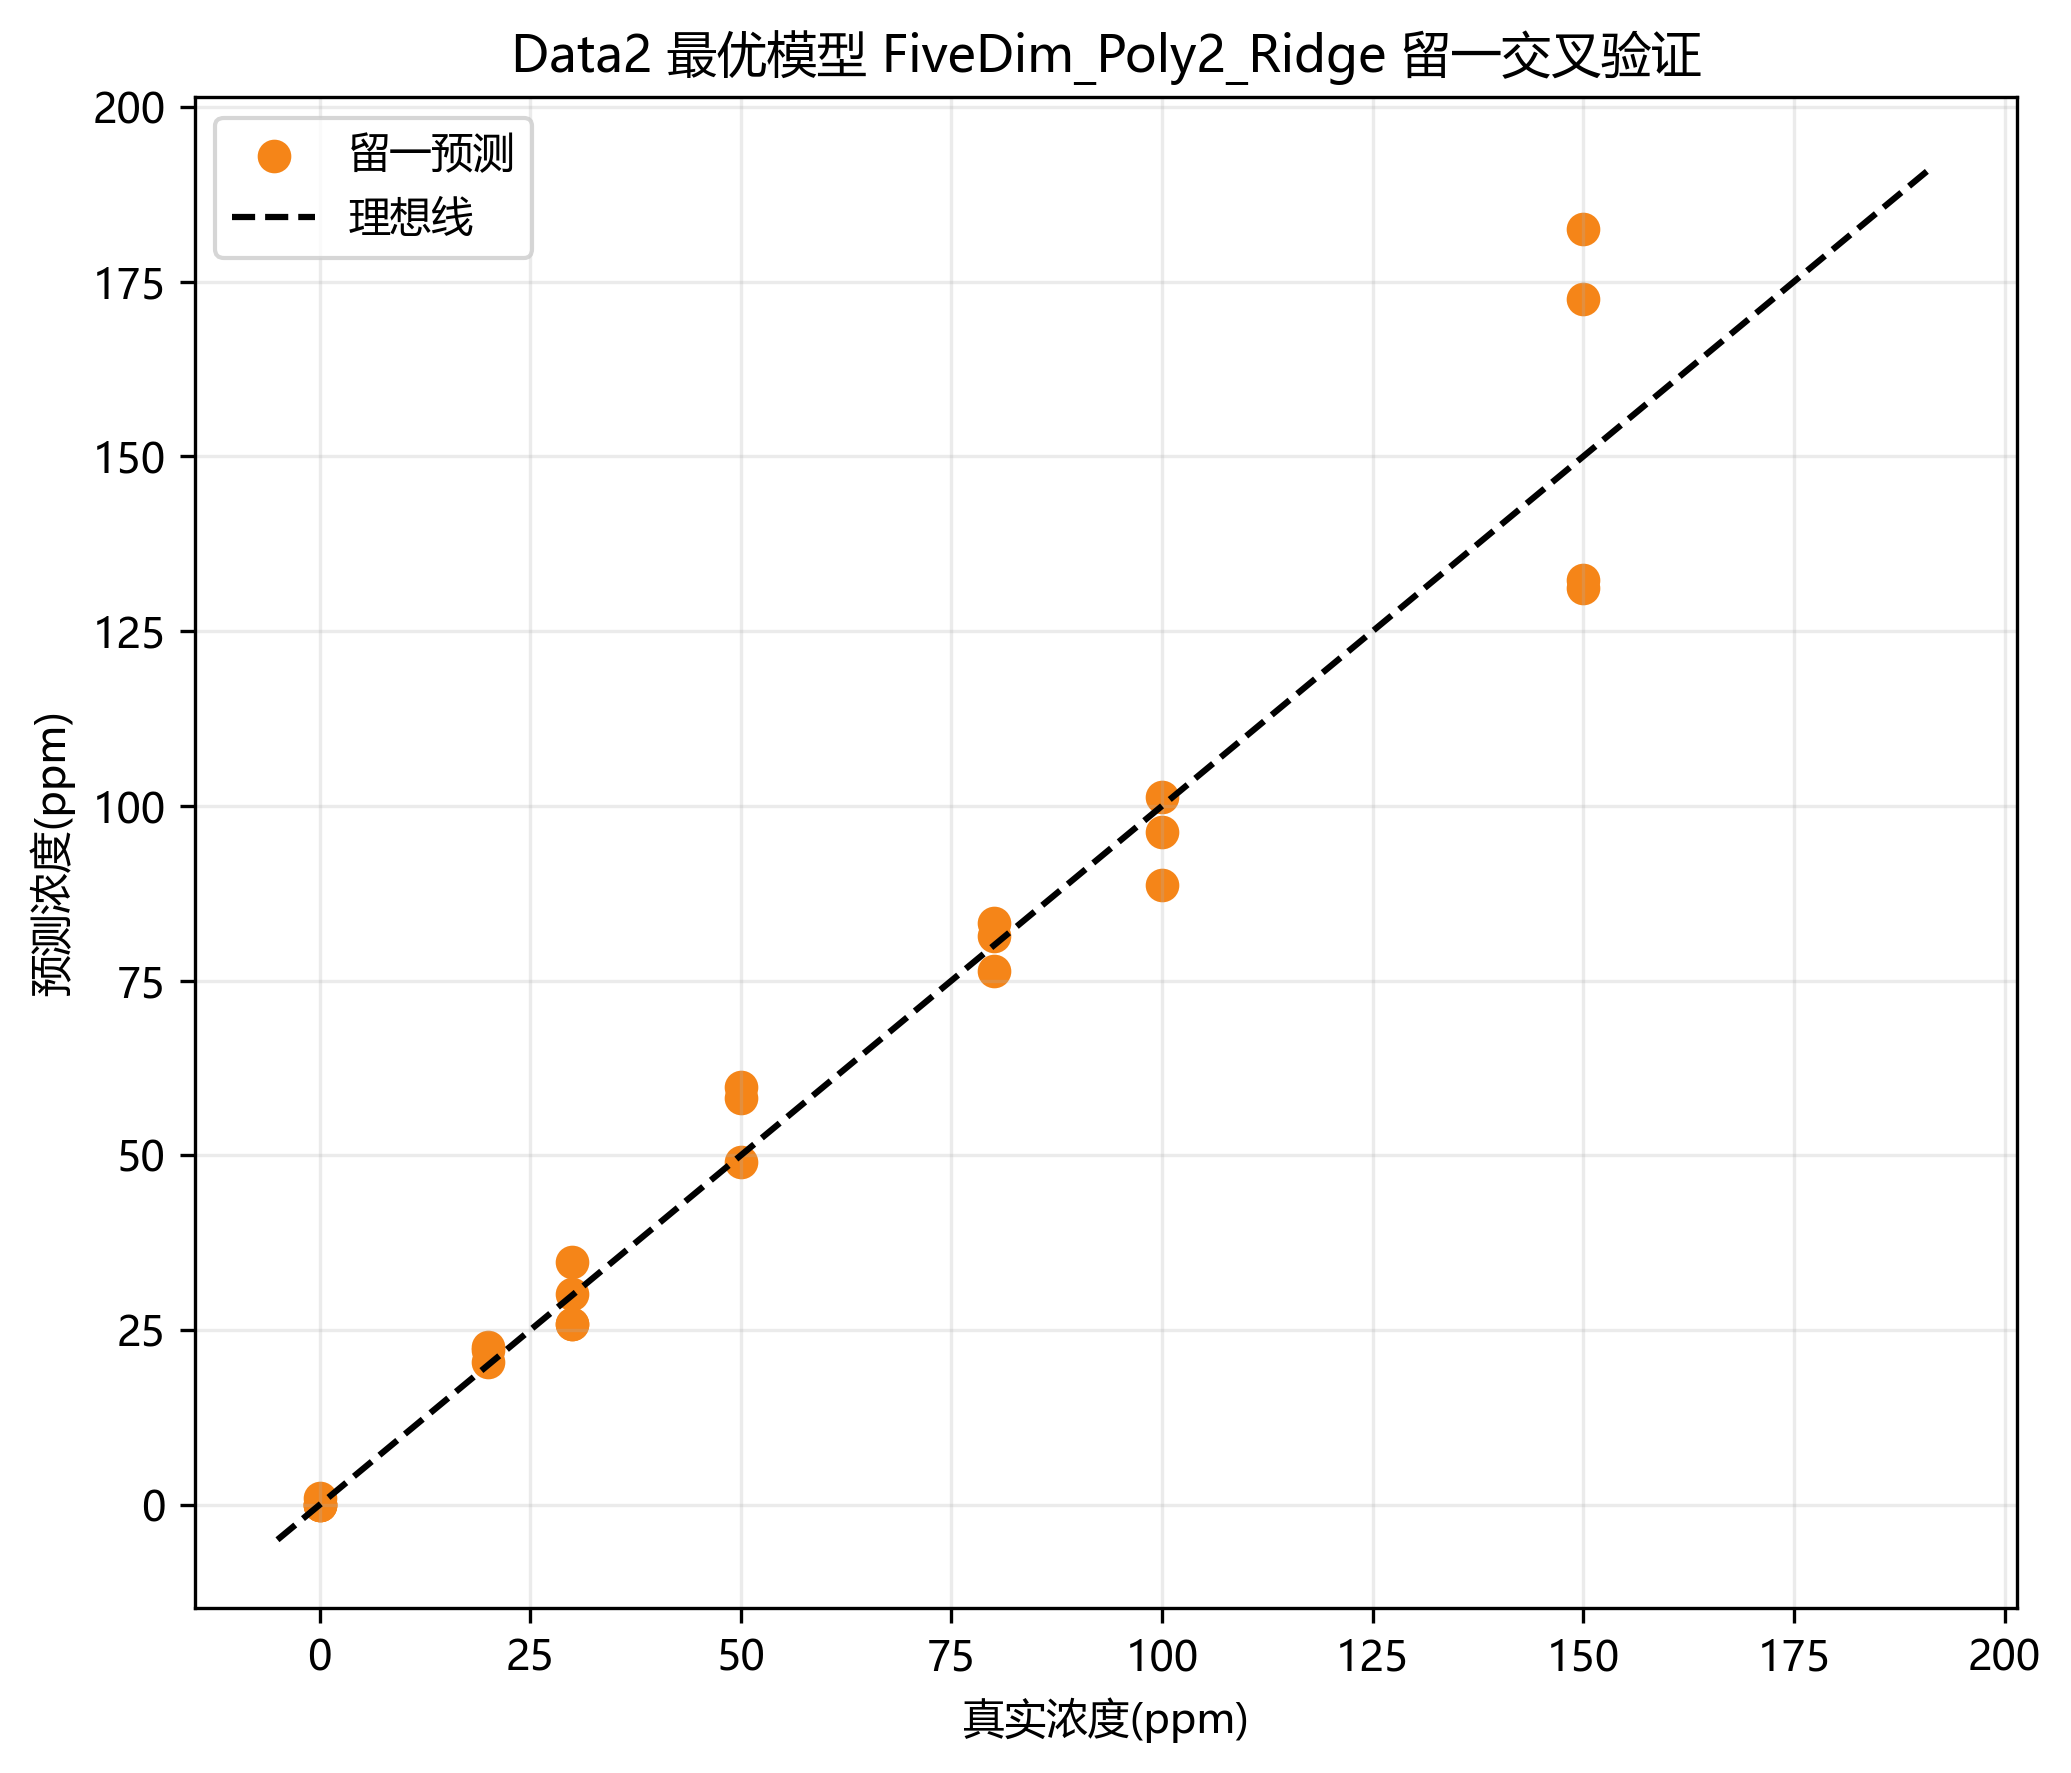
\includegraphics[width=.78\textwidth]{问题2_真实预测对比.png}\caption{最优模型真实浓度与留一预测浓度对比}\end{figure}
图中大多数点靠近理想线，说明模型在 20--100 ppm 区间预测较好。高浓度 150 ppm 处存在一定偏差，这与高浓度样本较少和颜色响应可能趋于饱和有关。
\begin{table}[H]\centering\small\caption{不同浓度水平下颜色均值、预测均值与误差}\begin{tabular}{rrrrrr}\toprule
浓度 & 样本数 & R均值 & G均值 & H均值 & MAE\\\midrule
0 & 5 & 153.4 & 146.4 & 17.8 & 0.02\\
20 & 3 & 144.3 & 115.0 & 82.0 & 6.41\\
30 & 4 & 145.3 & 114.0 & 88.5 & 5.21\\
50 & 3 & 141.7 & 99.0 & 109.7 & 5.54\\
80 & 3 & 140.7 & 96.0 & 119.3 & 4.89\\
100 & 3 & 139.0 & 96.0 & 115.0 & 4.76\\
150 & 4 & 138.8 & 86.3 & 130.5 & 21.06\\
\bottomrule\end{tabular}\end{table}
\begin{figure}[H]\centering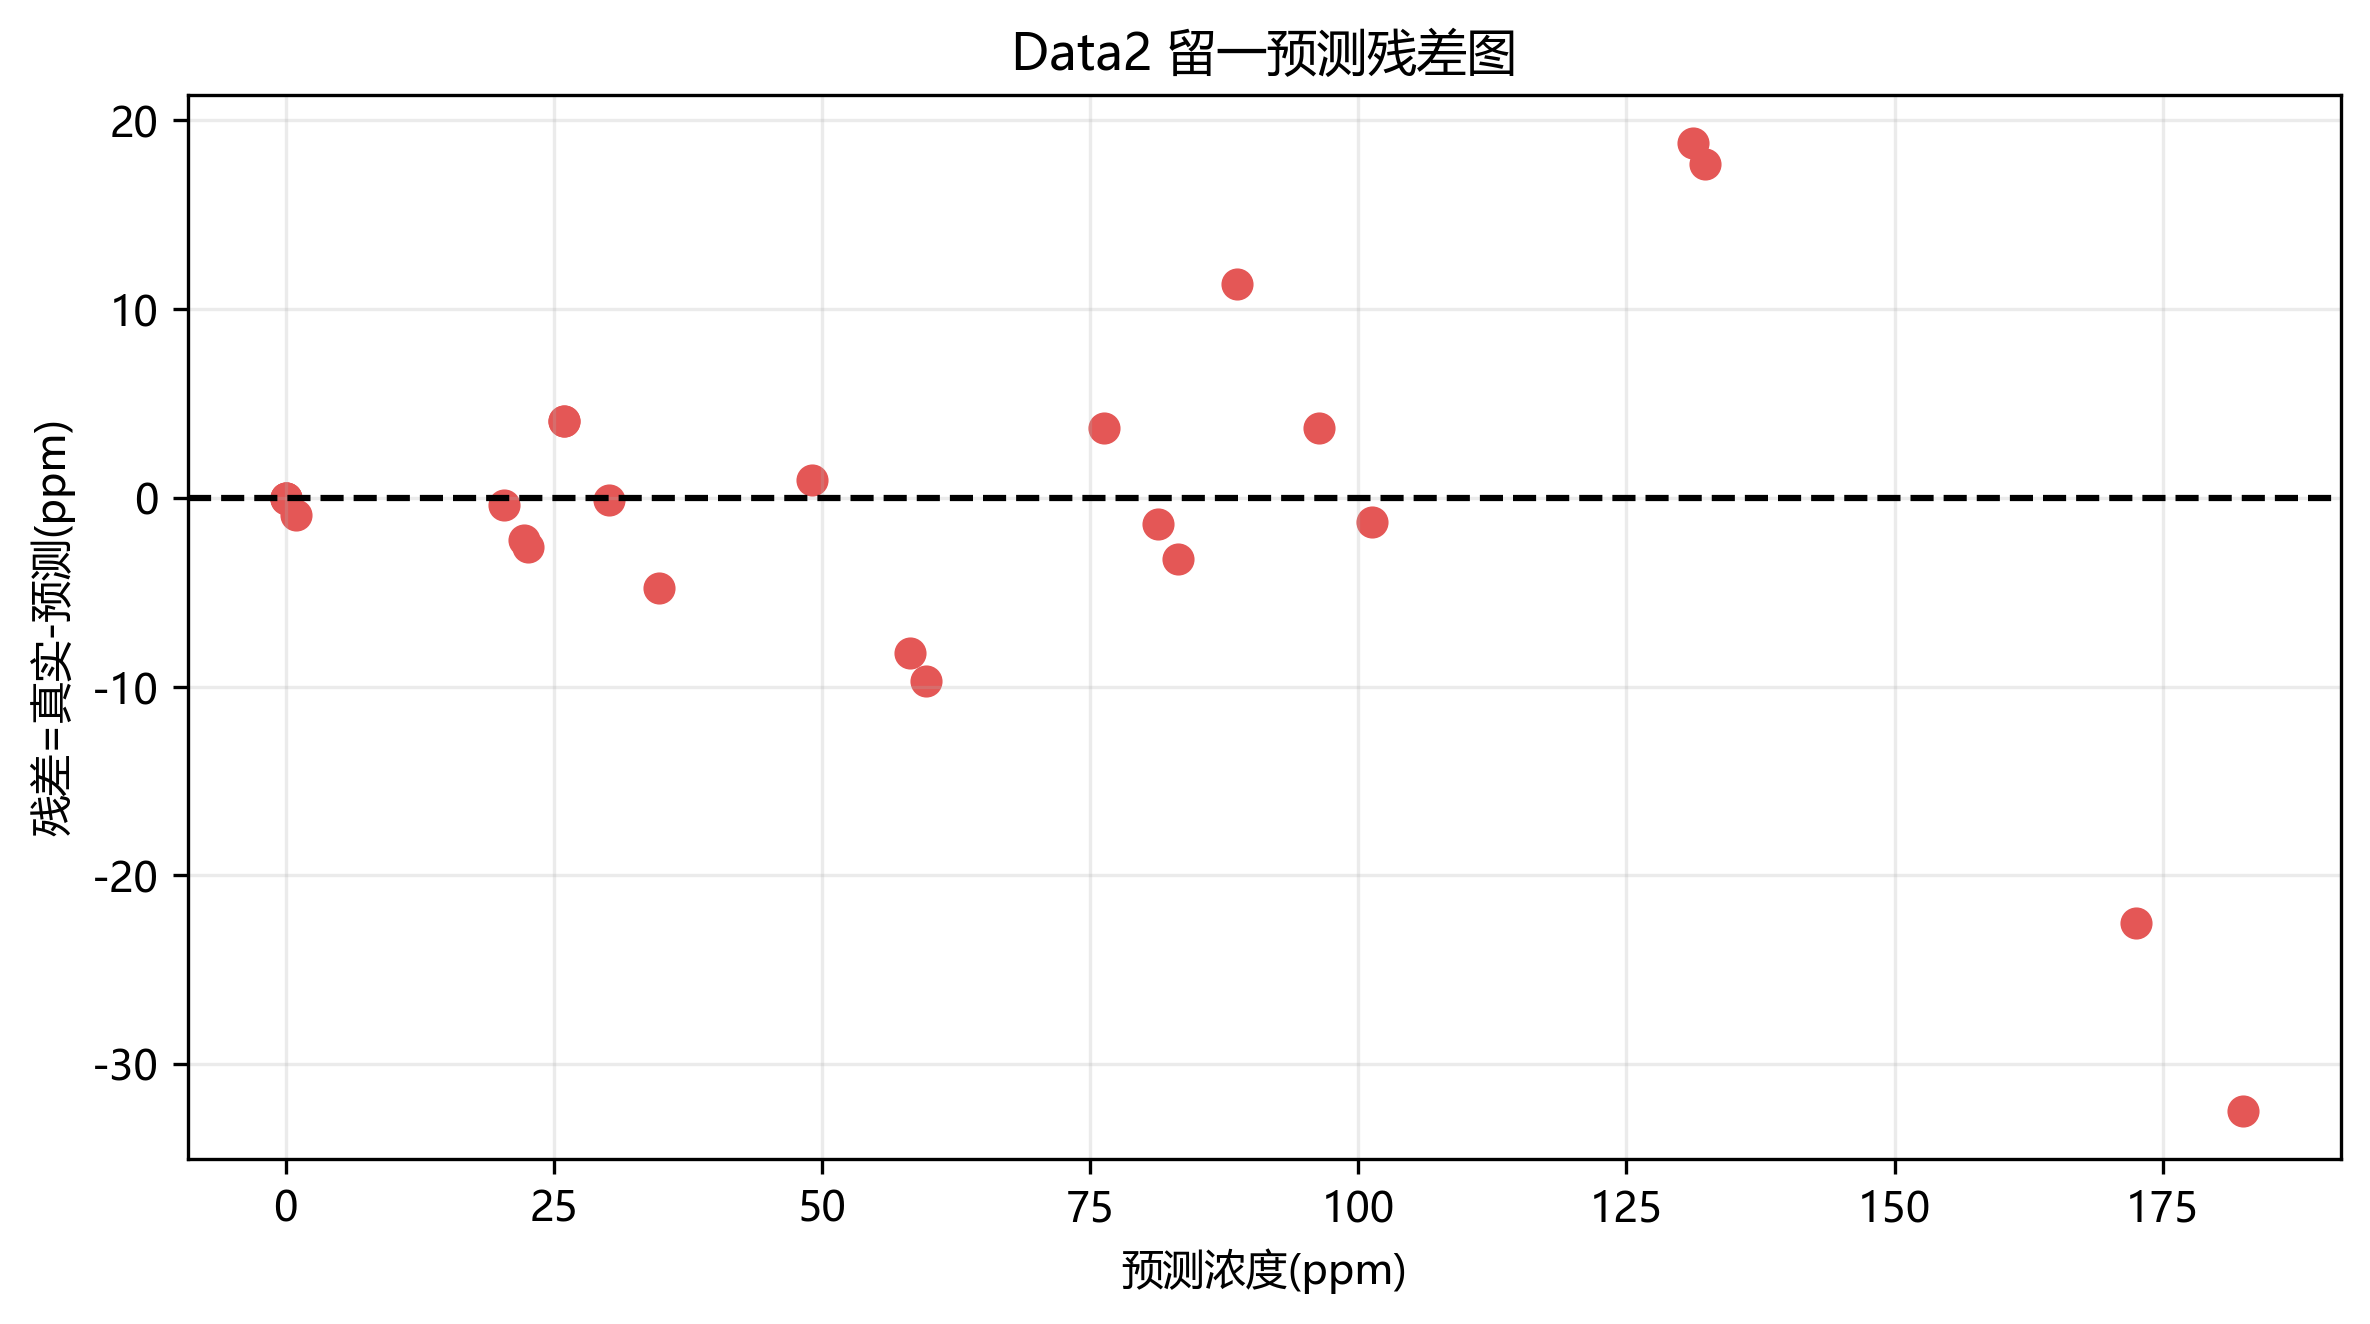
\includegraphics[width=.78\textwidth]{问题2_残差图.png}\caption{留一预测残差图}\end{figure}
残差均值为 -1.03 ppm，接近 0；残差标准差为 10.41 ppm，最大绝对误差为 32.48 ppm。残差随预测浓度增大而略有扩散，提示高浓度端存在异方差风险。
\begin{figure}[H]\centering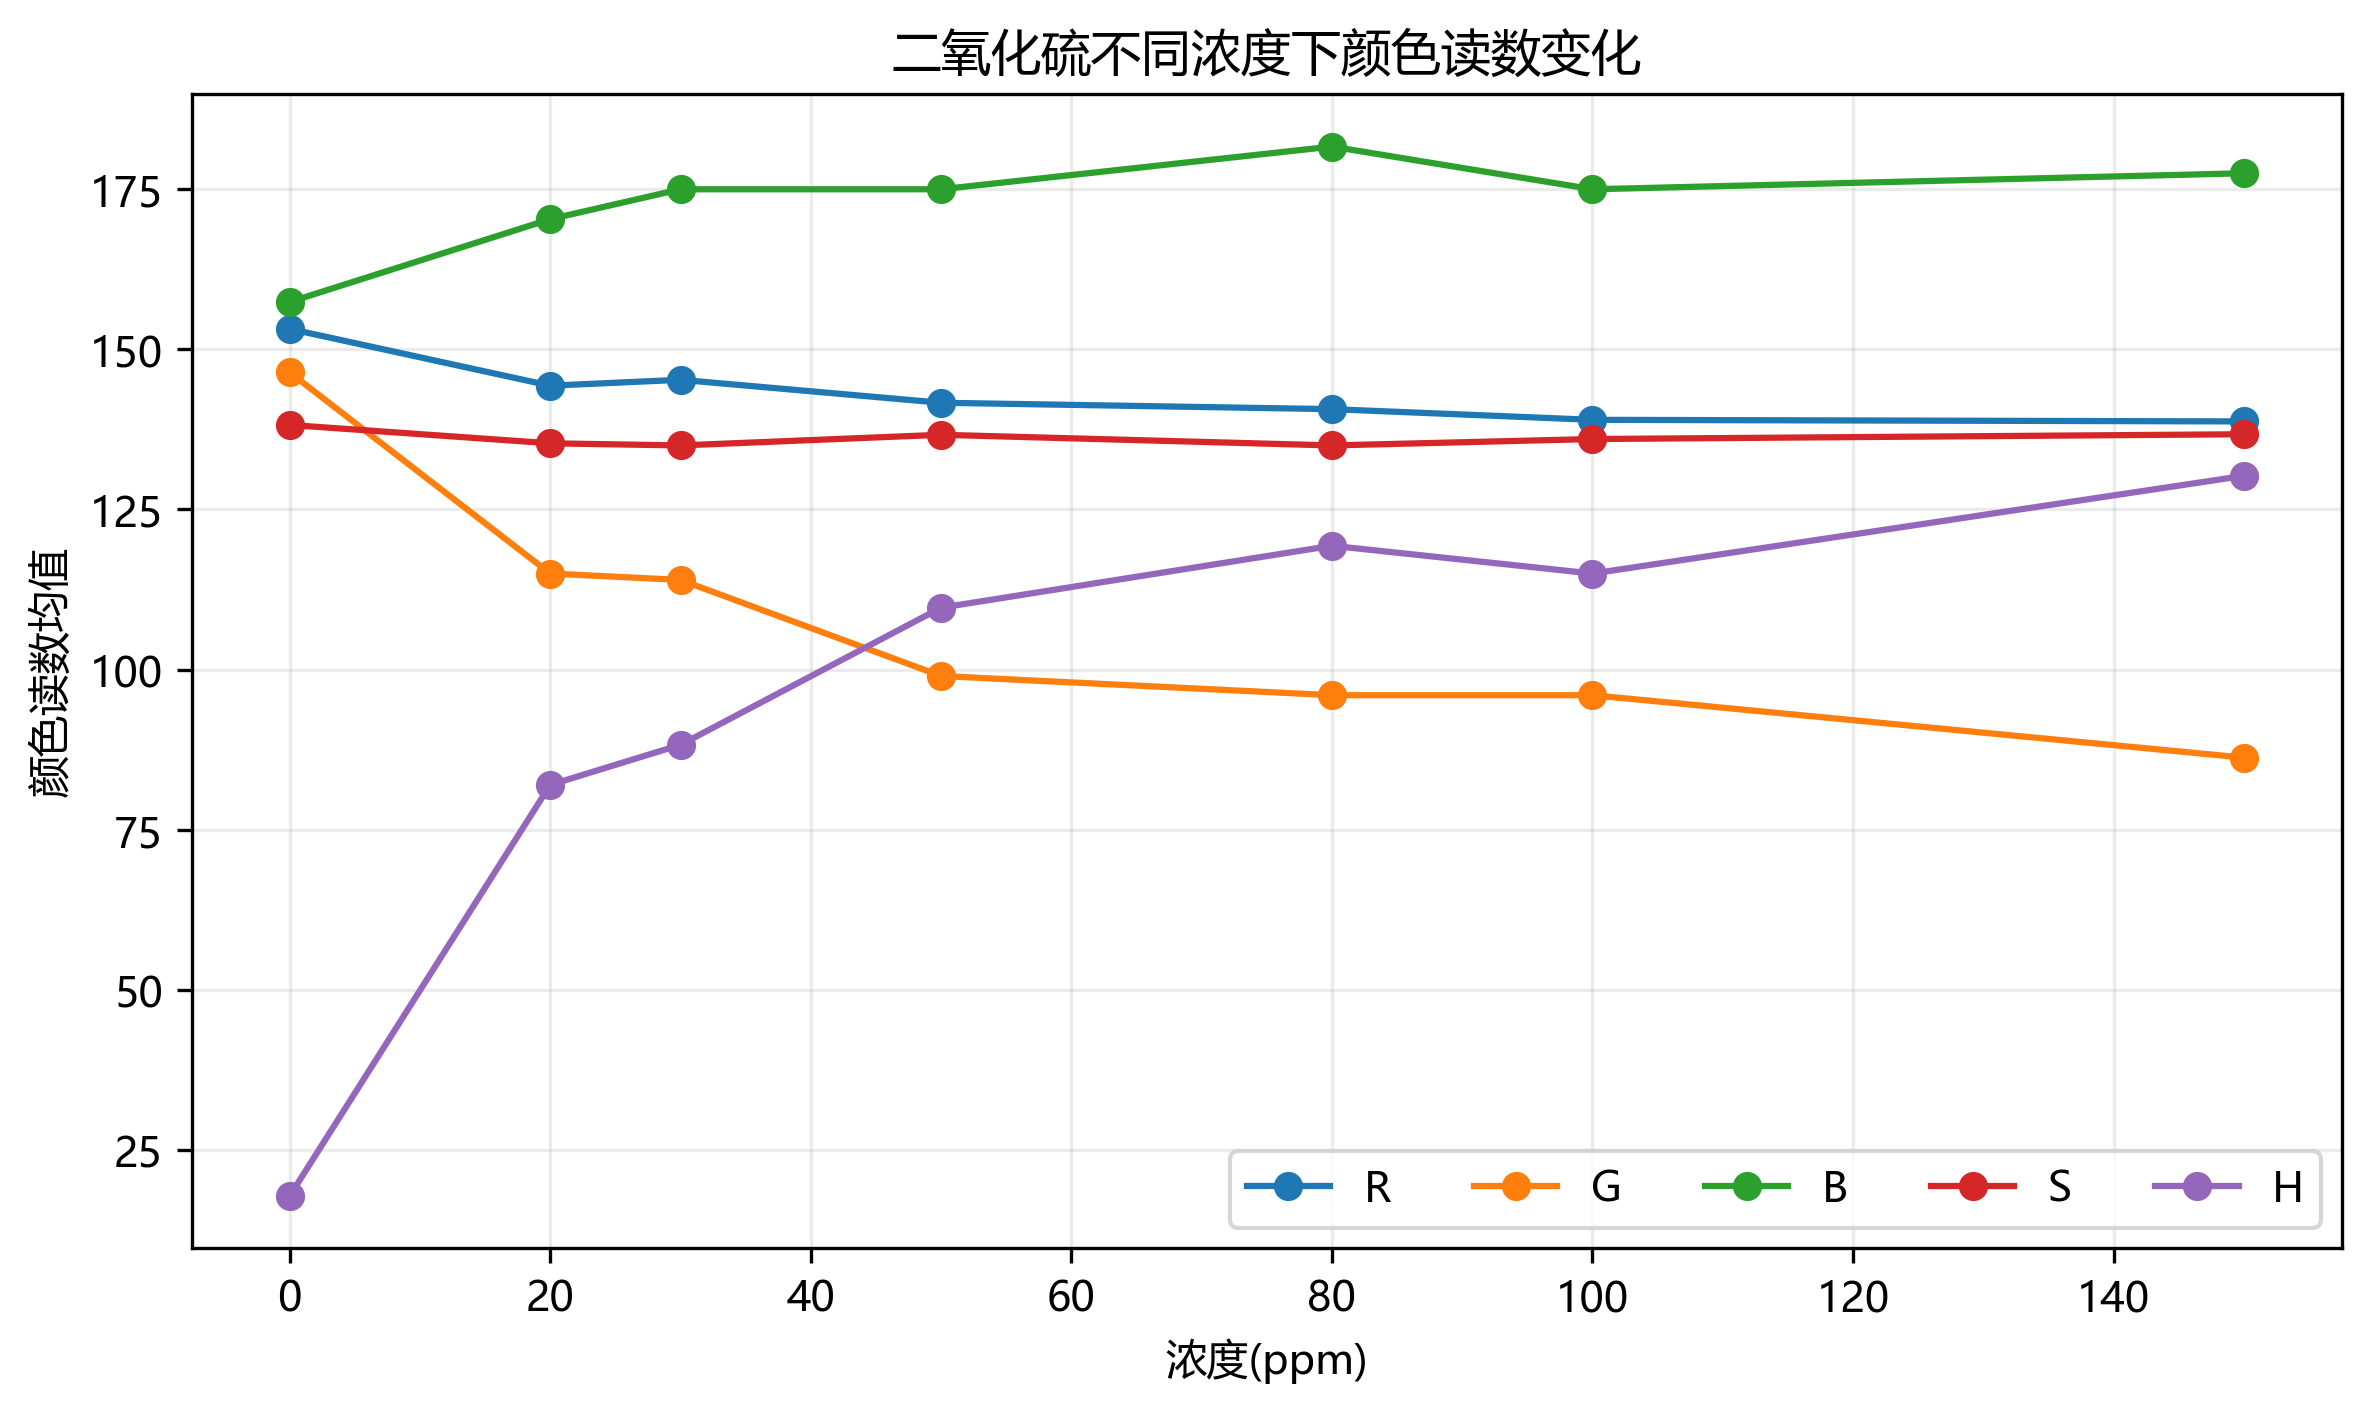
\includegraphics[width=.86\textwidth]{问题2_颜色维度随浓度变化.png}\caption{二氧化硫不同浓度下颜色读数变化}\end{figure}
\subsection{问题三：数据量与颜色维度影响}
为研究数据量影响，本文分别取约 35\%、50\%、70\%、90\% 和 100\% 样本重复抽样，并在每个子样本上进行留一交叉验证。样本比例小于 1 时重复 40 次，报告 RMSE 均值和标准差。
\begin{table}[H]\centering\small\caption{样本量与颜色维度对 RMSE 的影响}\begin{tabular}{lrrr}\toprule
维度 & 样本比例 & 样本数 & RMSE均值\\\midrule
D0 & 0.35 & 8 & 25.08\\ RGB & 0.35 & 8 & 31.27\\ HSV & 0.35 & 8 & 26.81\\ RGBSH & 0.35 & 8 & 39.50\\
D0 & 0.70 & 17 & 16.54\\ RGB & 0.70 & 17 & 24.73\\ HSV & 0.70 & 17 & 16.35\\ RGBSH & 0.70 & 17 & 19.90\\
D0 & 1.00 & 25 & 13.71\\ RGB & 1.00 & 25 & 15.30\\ HSV & 1.00 & 25 & 12.63\\ RGBSH & 1.00 & 25 & 10.60\\
\bottomrule\end{tabular}\end{table}
完整样本下，RGBSH 五维组合 RMSE 为 10.60 ppm，是四类维度中最优。
\begin{figure}[H]\centering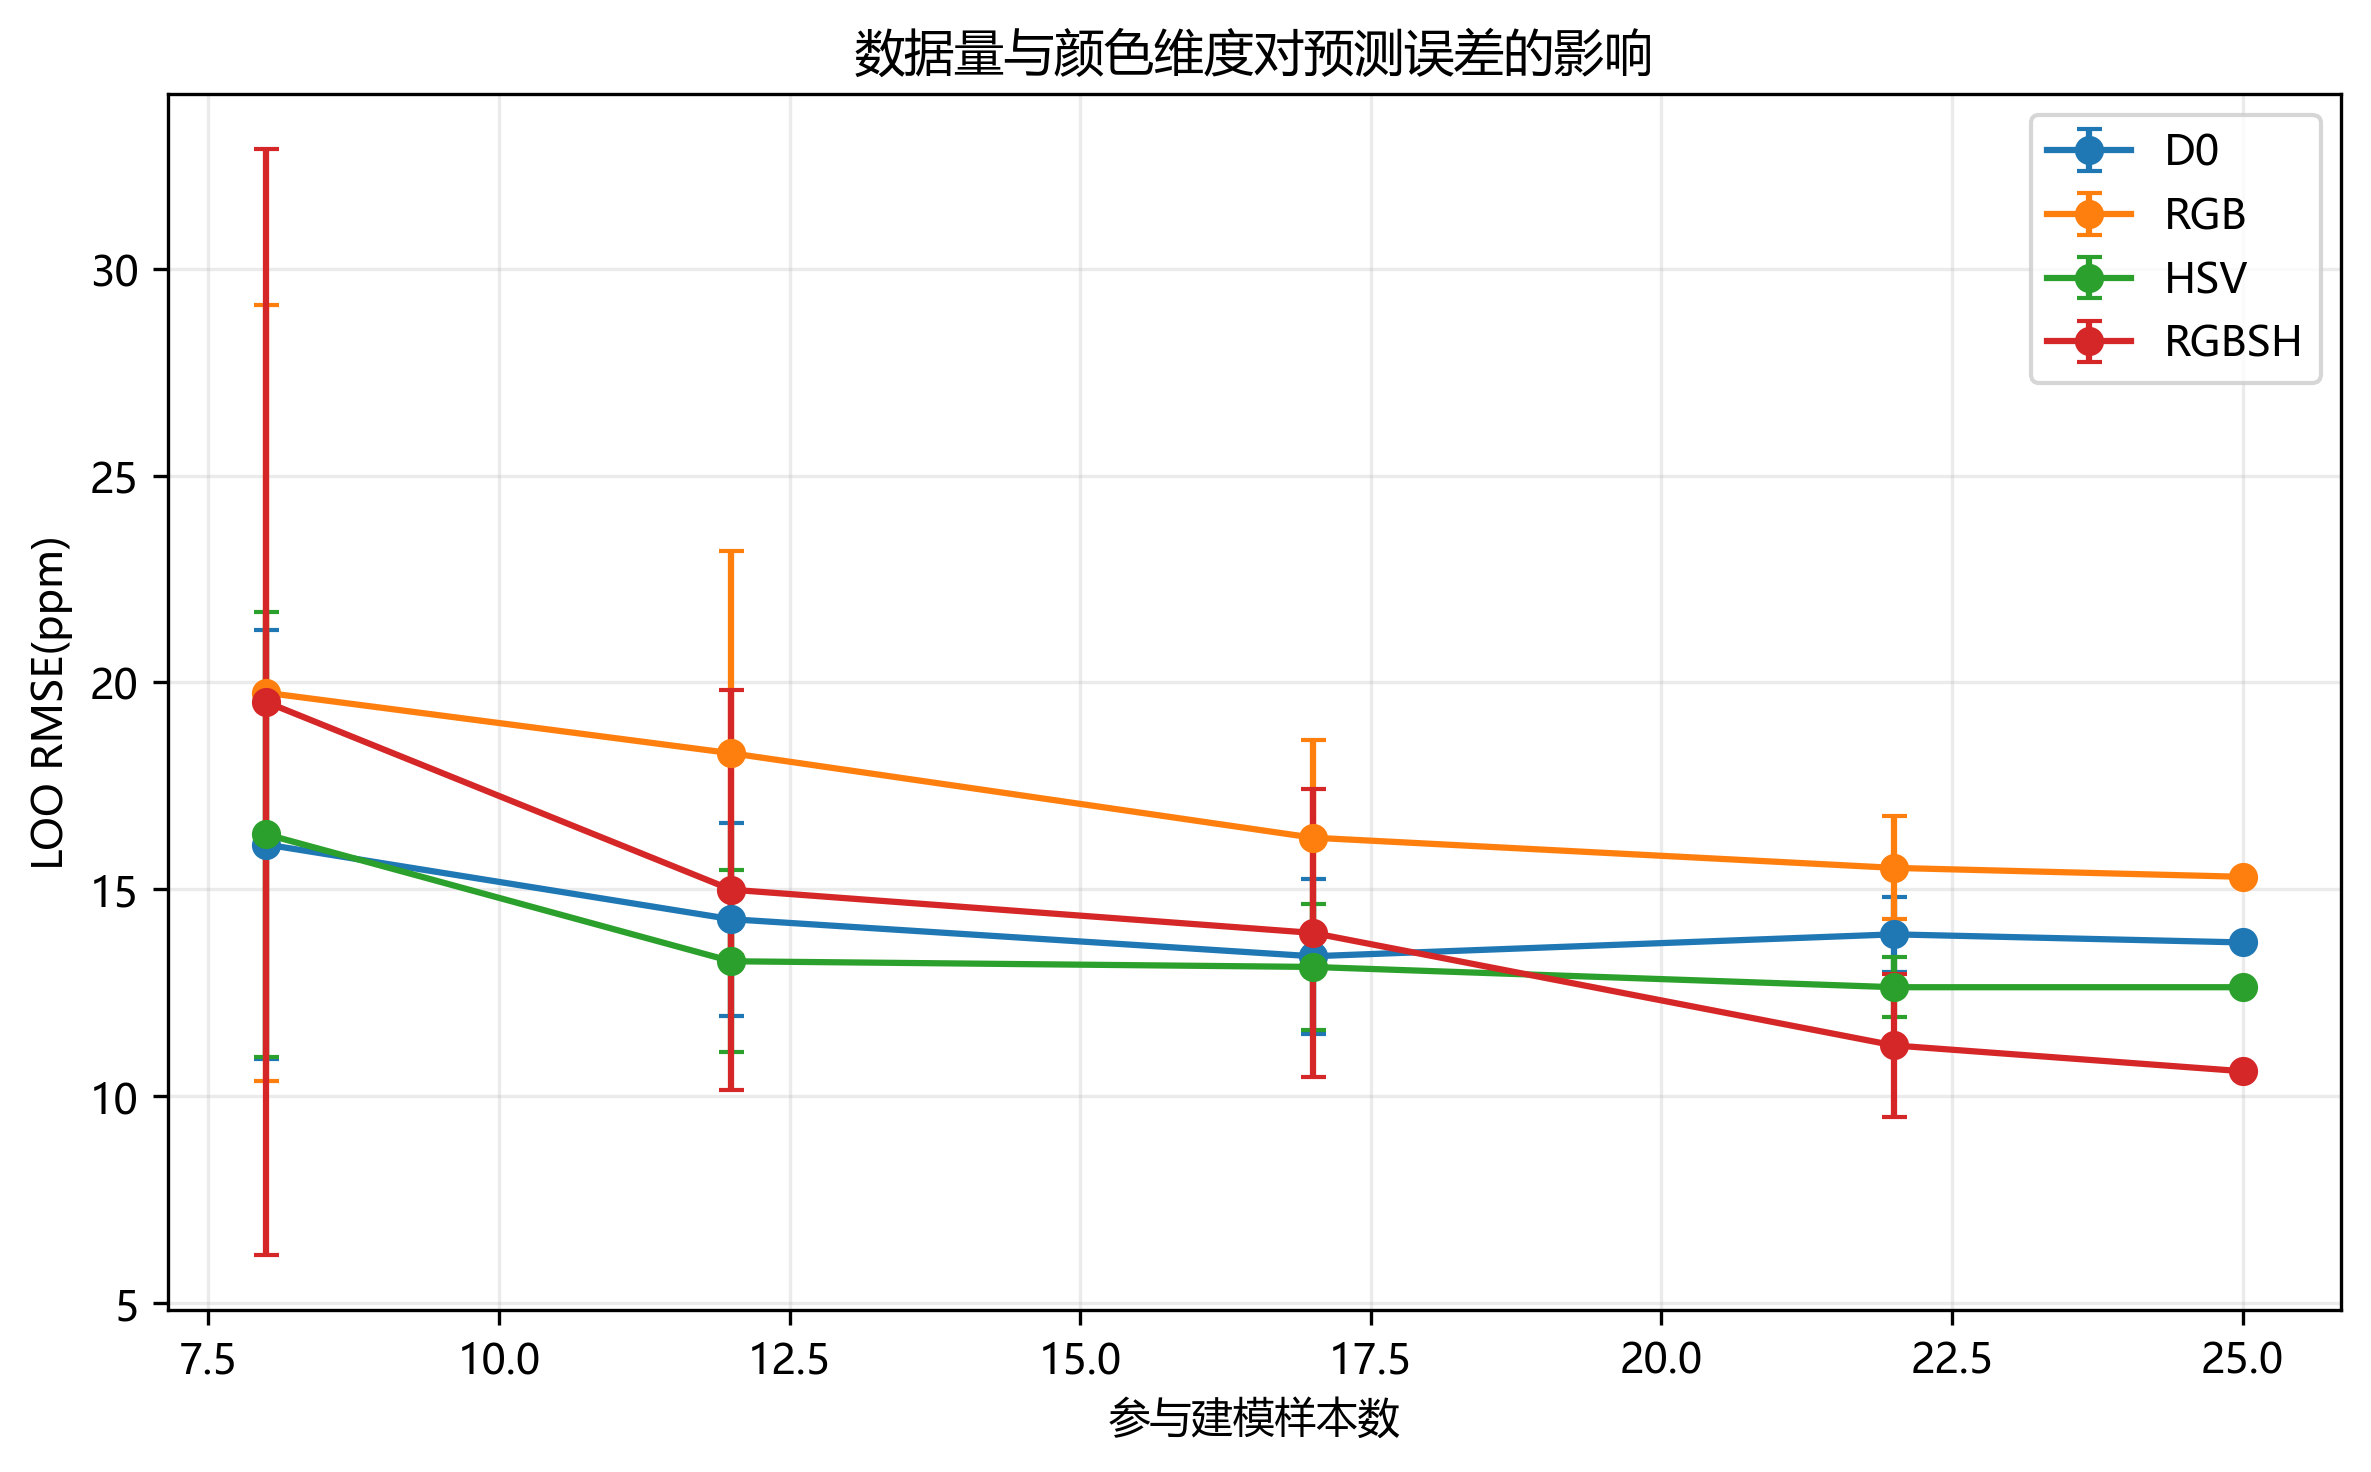
\includegraphics[width=.84\textwidth]{问题3_数据量颜色维度影响.png}\caption{数据量与颜色维度对预测误差的影响}\end{figure}
\begin{table}[H]\centering\small\caption{颜色维度重要性与相关性}\begin{tabular}{lrr}\toprule
维度 & 置换重要性 & Spearman相关\\\midrule
R & 0.157 & -0.893\\ G & 0.122 & -0.905\\ B & 0.115 & 0.706\\ S & 0.101 & -0.105\\ H & 0.363 & 0.878\\
\bottomrule\end{tabular}\end{table}
置换重要性和 Spearman 相关共同表明，H 维度对二氧化硫浓度辨识贡献最高。若实际设备只能记录有限维度，优先保留 H、G、B 等响应明显的维度。
\begin{figure}[H]\centering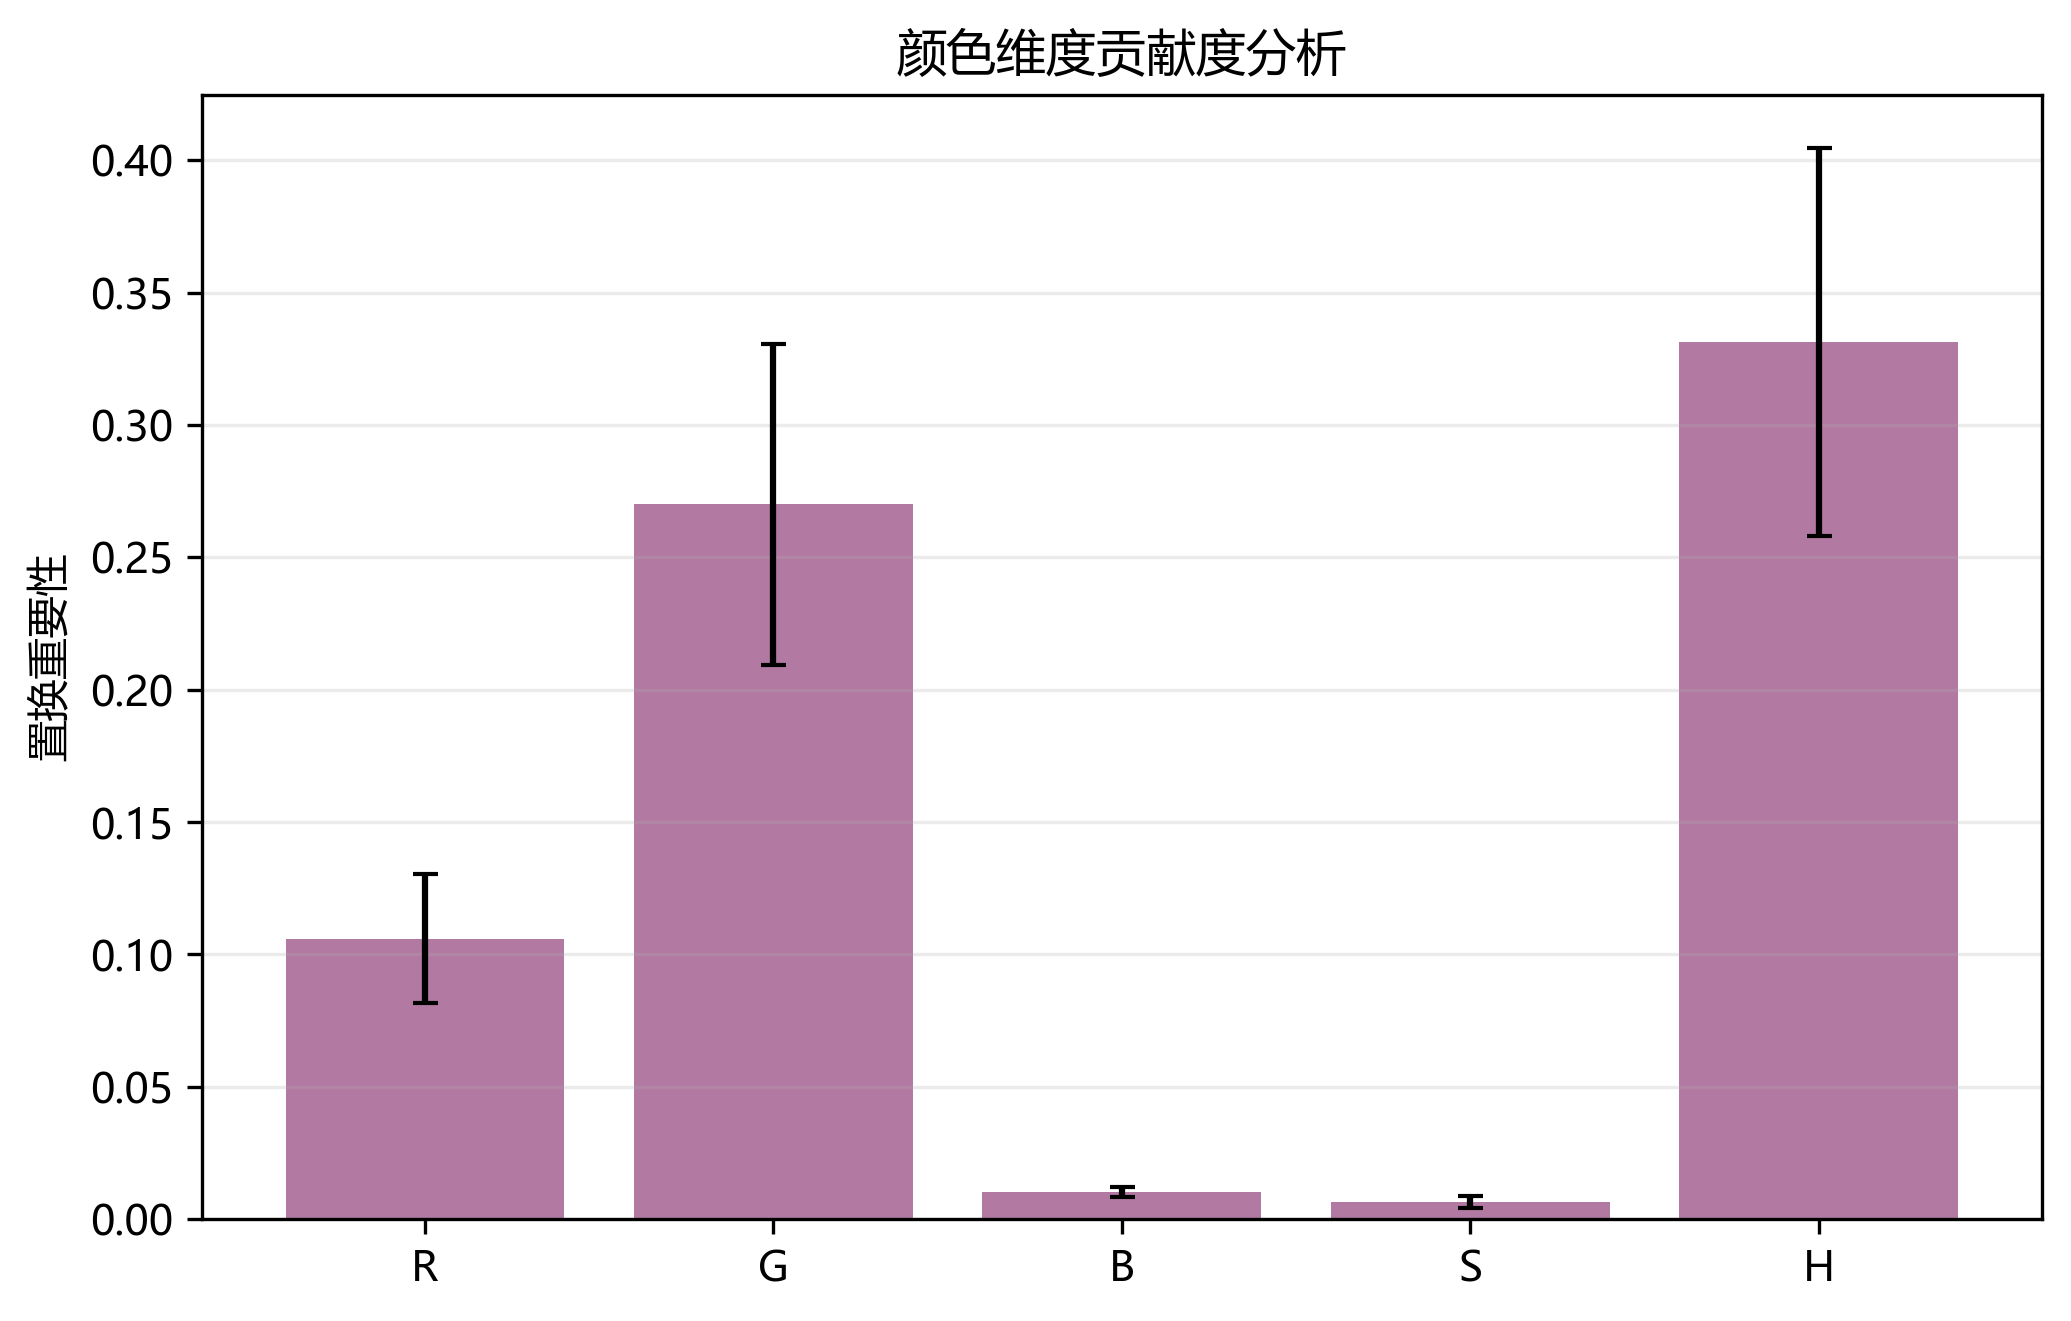
\includegraphics[width=.76\textwidth]{问题3_颜色维度贡献度.png}\caption{颜色维度贡献度}\end{figure}
\begin{table}[H]\centering\small\caption{颜色读数噪声敏感性分析}\begin{tabular}{rrr}\toprule
噪声标准差 & RMSE均值 & RMSE标准差\\\midrule
0 & 10.60 & 0.00\\ 1 & 14.68 & 5.31\\ 2 & 16.27 & 6.34\\ 3 & 18.40 & 7.65\\ 5 & 23.73 & 10.44\\ 8 & 33.64 & 14.64\\
\bottomrule\end{tabular}\end{table}
当颜色读数噪声标准差由 0 增加到 5 时，RMSE 从 10.60 ppm 上升到 23.73 ppm，说明模型对拍照条件和读数误差较敏感。
\begin{figure}[H]\centering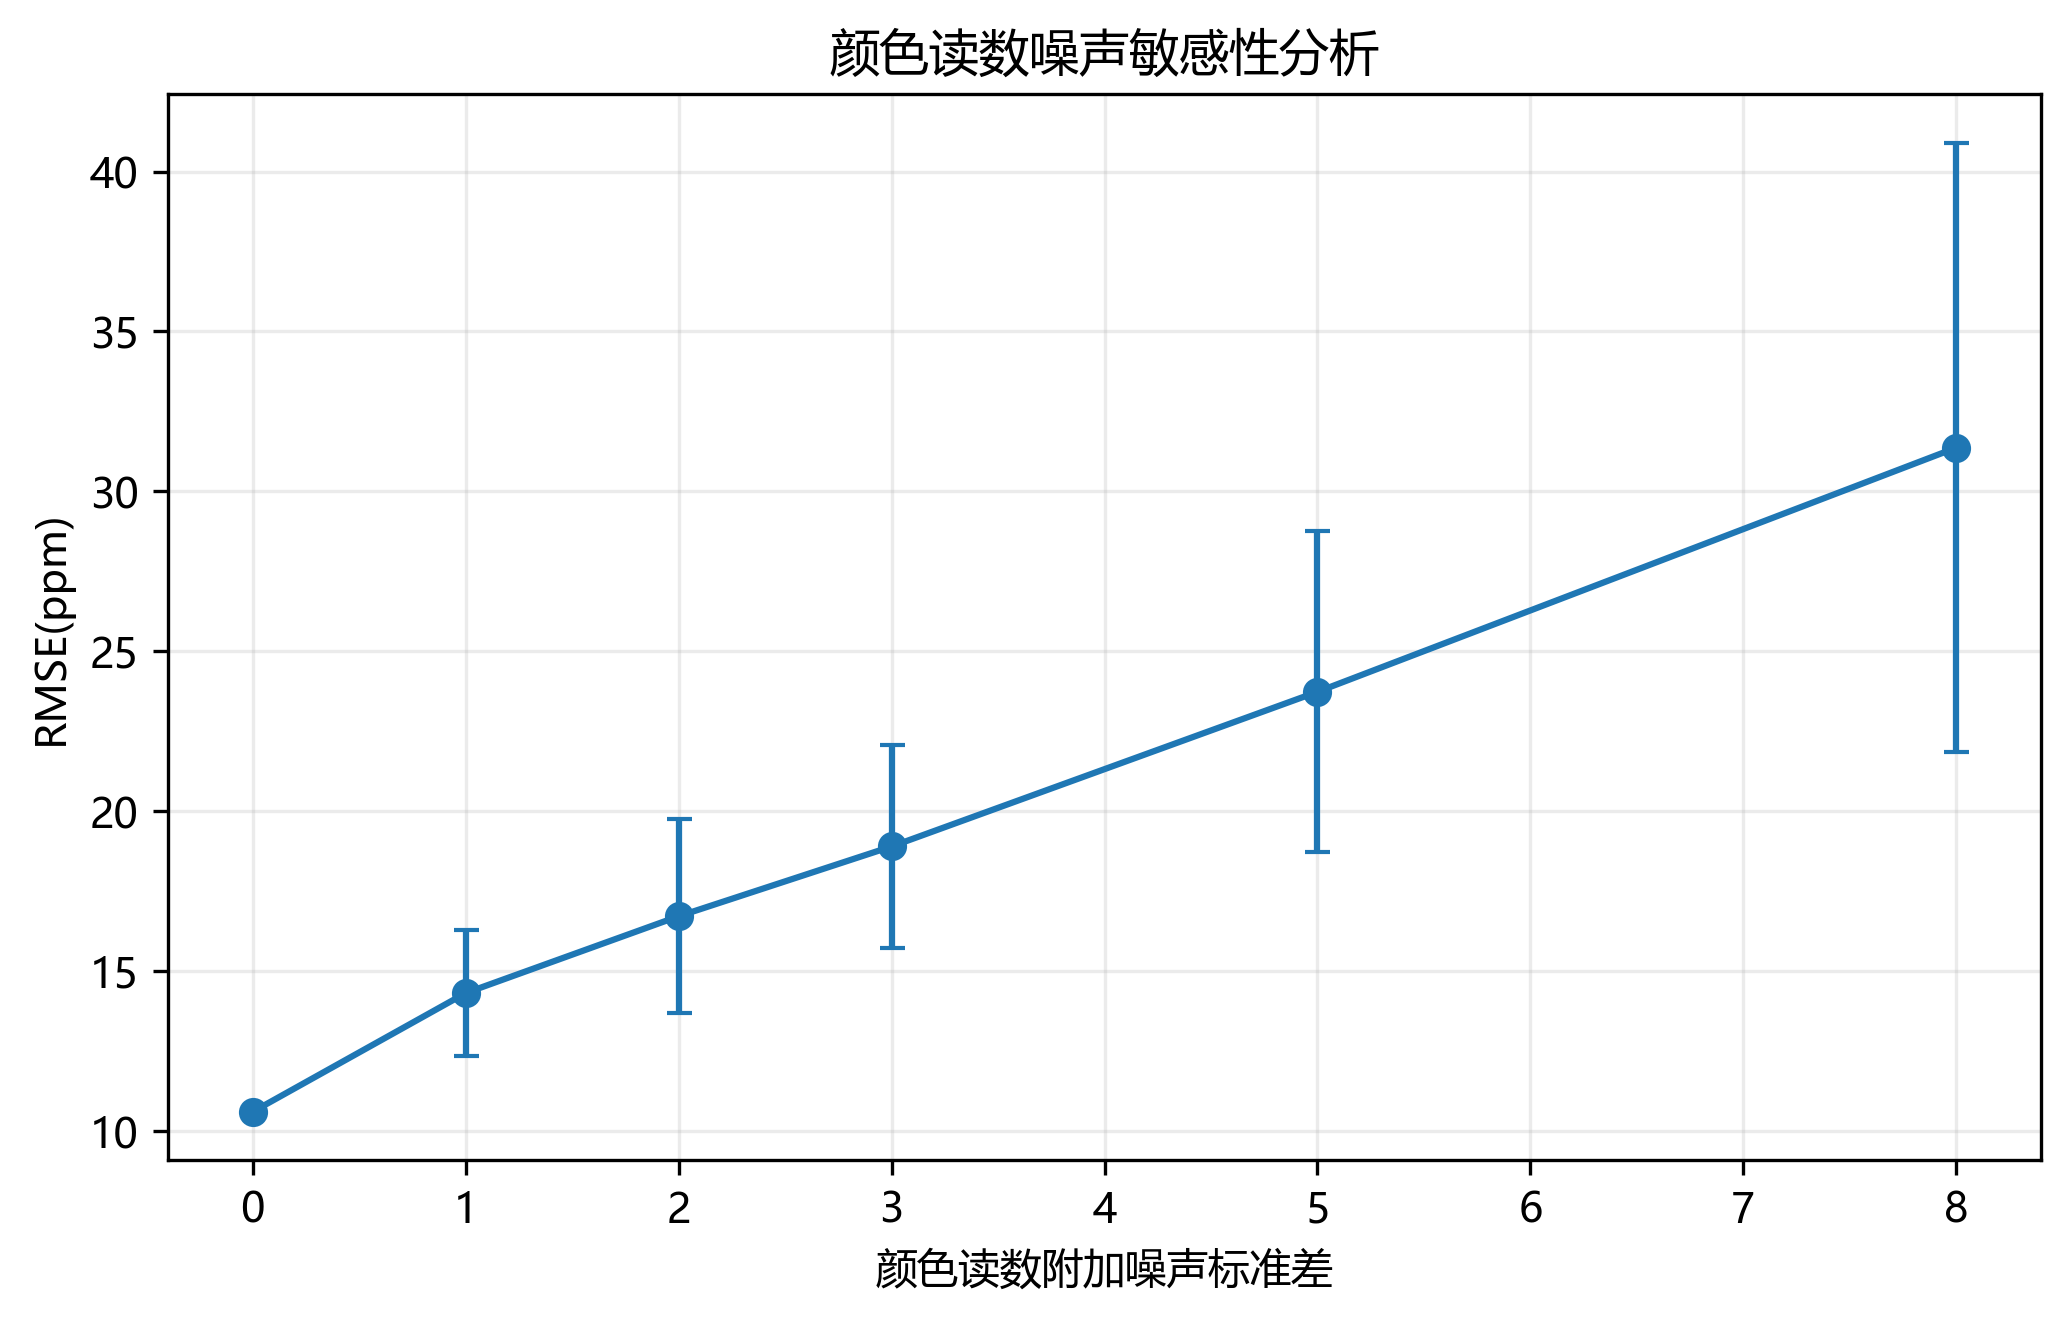
\includegraphics[width=.76\textwidth]{问题3_颜色噪声敏感性.png}\caption{颜色读数噪声敏感性曲线}\end{figure}
\section{模型检验与稳健性分析}
\subsection{Baseline 对比}
本文每个主模型均设置 baseline。问题一的 baseline 是单一颜色维度或 $D_0$ 与浓度的直接单调关系；问题二的 baseline 是 $D_0$ 一元线性回归。最终模型在 Data2 上 RMSE 从 13.71 ppm 降至 10.25 ppm，说明引入多维颜色信息和二次项有实际收益，而不是单纯增加模型复杂度。
\subsection{交叉验证检验}
由于 Data2 样本量小，本文采用留一交叉验证。每个样本仅在未参与训练的情况下预测一次，因此误差可以近似反映小样本泛化能力。最优模型 $R^2=0.960$，说明模型解释了大部分浓度变化。MAPE=9.75\%，表示在非零浓度样本上的平均相对误差约为 10\% 左右。
\subsection{残差与敏感性检验}
残差均值接近零，说明模型整体无明显偏移；残差图中高浓度区域误差略大，说明颜色响应在高浓度端可能接近饱和，且 150 ppm 样本数量有限。敏感性分析显示，小样本抽样时误差波动较大；颜色读数噪声标准差增大后 RMSE 明显上升。因此本文模型的可靠性依赖于足够标定样本和稳定拍照条件。
\section{模型评价、改进与推广}
\subsection{模型优点}
第一，本文模型具有明确的题意对齐。问题一不是直接套用回归，而是先判断数据是否适合建模；问题二建立可复现的浓度预测模型；问题三进一步分析数据量和维度对模型的影响。三个子问题形成从数据质量到模型建立再到实验设计建议的闭环。

第二，模型兼顾可解释性与预测精度。相对白板色差 $D_0$ 具有明确物理含义；岭回归和 PLS 回归适合小样本多变量问题；二次岭回归允许适度非线性，同时通过正则化抑制过拟合。

第三，验证较完整。本文没有只报告训练拟合效果，而是使用留一交叉验证、baseline 对比、残差分析、维度消融和噪声敏感性分析，保证结果可审计。
\subsection{模型局限}
第一，样本量仍偏小，Data2 只有 25 个有效样本，且高浓度端样本数量有限，导致模型在 150 ppm 位置误差较大。第二，本文没有显式引入照明、试纸反应时间、相机型号等外部因素。若实际拍摄条件发生明显变化，即使浓度相同，颜色读数也可能偏移。第三，模型主要建立在统计相关关系上，没有深入刻画化学显色反应的动力学机制。
\subsection{改进与推广}
未来可以增加标定样本，特别是在 0--30 ppm 和 100--180 ppm 等关键区间增加重复浓度点；采集拍摄条件变量，例如光源色温、曝光、白平衡和试纸反应时间；建立分段或饱和型响应模型，例如 Logistic、Michaelis--Menten 型函数或样条回归。本文方法可推广到食品安全、环境监测等其他比色检测任务。
\section{结论}
\begin{enumerate}
\item Data1 五组数据中，溴酸钾综合质量最好，得分 91.64；工业碱和组胺也适合建立颜色--浓度关系；奶中尿素得分最低，为 52.91，不宜直接建立高精度定量模型。
\item Data2 二氧化硫最优模型为五维二次岭回归，留一 RMSE=10.25 ppm，MAE=6.17 ppm，MAPE=9.75\%，$R^2=0.960$，优于 $D_0$ 一元 baseline。
\item 数据量不足会增加误差波动；完整样本下 RGBSH 五维组合误差最低。H 维度贡献最高，说明色调信息对二氧化硫显色响应十分重要。
\item 颜色读数噪声会显著放大预测误差，因此实际应用应统一光照、白平衡和拍摄距离，并通过重复拍照取均值提高稳定性。
\end{enumerate}
\begin{thebibliography}{9}
\bibitem{colorimetry} Gonzalez R C, Woods R E. Digital Image Processing[M]. 4th ed. Pearson, 2018.
\bibitem{regression} Hastie T, Tibshirani R, Friedman J. The Elements of Statistical Learning[M]. Springer, 2009.
\bibitem{pls} Wold S, Sjostrom M, Eriksson L. PLS-regression: a basic tool of chemometrics[J]. Chemometrics and Intelligent Laboratory Systems, 2001, 58(2):109-130.
\bibitem{ridge} Hoerl A E, Kennard R W. Ridge regression: biased estimation for nonorthogonal problems[J]. Technometrics, 1970, 12(1):55-67.
\bibitem{sklearn} Pedregosa F, et al. Scikit-learn: Machine Learning in Python[J]. Journal of Machine Learning Research, 2011, 12:2825-2830.
\bibitem{cumcm} 全国大学生数学建模竞赛组织委员会. 全国大学生数学建模竞赛论文格式规范[EB/OL].
\end{thebibliography}
\appendix
\section{支撑材料与复现说明}
支撑材料目录包含 \texttt{data/} 原始数据，\texttt{code/main\_modeling.py} 主程序，\texttt{tables/} 结果表，\texttt{results/frozen\_numbers.json} 冻结数字，\texttt{quest1/figures}、\texttt{quest2/figures}、\texttt{quest3/figures} 图表，以及 \texttt{papper/论文.tex} 和 \texttt{papper/论文.pdf}。复现命令为：\texttt{python 支撑材料/code/main\_modeling.py}，然后在 \texttt{papper} 目录运行三遍 \texttt{xelatex 论文.tex}。
\section{核心代码入口}
完整代码见支撑材料 \texttt{code/main\_modeling.py}。该程序完成 Excel 解析、数据清洗、质量评价、模型训练、留一交叉验证、图表保存和冻结数字写入。所有图表均使用 \texttt{plt.savefig(..., dpi=300)} 与 \texttt{plt.close()} 保存，没有使用交互式窗口。
\section{三层质量门控审计}
L1 建模合理性：通过。三个子问题均有题目要求与模型输出映射，假设服务于白板校正、分物质建模和噪声分析，问题二含 baseline 对比。\par
L2 求解正确性：通过。完成数据审计，代码固定随机种子，使用留一交叉验证，关键数字冻结。\par
L3 论文质量：通过。摘要含关键数字，图表均有编号和解释，公式与变量说明完整，PDF 经 XeLaTeX 编译并核验页数。
\end{document}
